\documentclass[10pt]{memoir}
\setstocksize{220mm}{155mm} 	        
\settrimmedsize{220mm}{155mm}{*}	
\settypeblocksize{170mm}{116mm}{*}	
\setlrmargins{18mm}{*}{*}
\setulmargins{*}{*}{1.2}
%\setlength{\headheight}{5pt}%
\checkandfixthelayout[lines]
\linespread{1.16}
\flushbottom

%%% Hyphenation settings
\usepackage[htt]{hyphenat}
\hyphenation{he-lio-trope opos-sum}
\tracingparagraphs=1
%Hyphenation in Devanāgarī of the edition still missing? Probably this needs to be modified in babel-iast package? 

%%% babel
\usepackage[english]{babel}
\usepackage{babel-iast/babel-iast}

\babelfont[iast]{rm}[Renderer=Harfbuzz, Scale=1.3]{AdishilaSan}%AdishilaSan}
\babelfont[english]{rm}{Adobe Text Pro}

%%% more functionality
\PassOptionsToPackage{hyphens}{url}
\usepackage{hyperref}
\usepackage{pdflscape}
\usepackage{cleveref}
\usepackage{url}
\usepackage{cleveref}
\usepackage{microtype}
\usepackage{lineno}

%\usepackage{bigfoot}
%%% more functions
\usepackage[dvipsnames]{xcolor}
%\usepackage[para,perpage]{footmisc}

%%%für den Counter von Kapiteln und Sätzen! 
\newcommand{\uproman}[1]{\uppercase\expandafter{\romannumeral#1}}
\newcommand{\lowroman}[1]{\romannumeral#1\relax}

\makeindex
\newfontfamily\sanskritfont[Script=Devanagari,Mapping=RomDev,Scale=1.1]{Sanskrit2003}
\usepackage{pifont,fourier-orns,lettrine,psvectorian,paralist,enumitem,pdfpages,wrapfig,tabulary,lettrine,longtable}
\setlist[enumerate]{itemsep=0mm}
\usepackage[autostyle]{csquotes}
\usepackage[defaultlines=2,all]{nowidow}
\usepackage{ellipsis,adforn,booktabs,longtable,url,tikz}
\lineskiplimit=-3pt          

\makechapterstyle{IeT}{%
  \chapterstyle{default}
  \renewcommand*{\printchapternonum}{\centering}
  \renewcommand*{\clearforchapter}{\cleartorecto} 
  \aliaspagestyle{chapter}{empty}}
\chapterstyle{IeT}
\setsecnumdepth{none}  \openright  \nouppercaseheads
\settocdepth{subsubsection}

%%%% test better pagebreaks
%\def\fussy{%
%  \emergencystretch\z@
%  \tolerance 200%
%  \hfuzz .1\p@
%  \vfuzz\hfuzz}

%\interfootnotelinepenalty=10000\relax

%\usepackage[maxfloats=256]{morefloats}

%\maxdeadcycles=500

%raggedbottomsectiontrue
%%\checkandfixthelayout


%%%%%%%  biblatex
%\newcommand{\noun}[1]{\textsc{#1}}    %  philosophy-verbose
\usepackage[backend=biber, sorting=nyt, style=verbose]{biblatex} %%%%ORIGINAL TiE
\renewcommand*{\mkbibnamefamily}[1]{\textsc{#1}}


\DeclareFieldFormat{url}{%
  \mkbibacro{URL}\addcolon\space
  \href{#1}{\nolinkurl{\thefield{urlraw}}}}

\DeclareFieldFormat{citeurl}{%
  \href{#1}{\nolinkurl{\thefield{urlraw}}}} 


\DeclareFieldFormat{postnote}{#1}
\renewcommand{\postnotedelim}{, }
\addbibresource{bindu.bib}

%%% ekdosis
\usepackage[teiexport=tidy,parnotes=true]{ekdosis}% =tidy cleans up HTML and XML documents by fixing markup errors and upgrading legacy code to modern standards. parnotes=footnotes below or above critical apparatus

\SetLineation{lineation=page, modulo} %lineation=page sets thenumbering to start afresh at the top of each page. =modulo makes every fifth line numbered. {lineation=page} makes every line numbered! 

\renewcommand{\linenumberfont}{\selectlanguage{english}\footnotesize} %sets language of lines to English

\SetTEIxmlExport{autopar=false} %autopar=falseinstructs ekdosis to ignore blank lines in the.tex sourcefile as markers for paragraph boundaries. As a result, each paragraph of the edition must be found within an environment associated with the xml <p> element

\SetHooks{
  lemmastyle=\bfseries,
  %refnumstyle=\selectlanguage{english}\bfseries,
  refnumstyle=\selectlanguage{english}\color{blue}\bfseries,
  appheight=0.8\textheight,
}

\newif\ifinapparatus
\DeclareApparatus{source}[
%bhook=\inapparatustrue,
lang=english,
notelang=english,
% bhook=\selectlanguage{english},
bhook=\selectlanguage{english}\textbf{Sources:},%
%maxentries=4, 
%ehook=.]
%sep={] },
%nosep,
]

\newif\ifinapparatus
\DeclareApparatus{testium}[
%bhook=\inapparatustrue,
lang=english,
notelang=english,
% bhook=\selectlanguage{english},
bhook=\selectlanguage{english}\textbf{Testimonia:},
%maxentries=4, 
%ehook=.]
%nosep, 
]

% Declare \ifinapparatus and set \inapparatustrue at the beginning of
% the apparatus criticus block. Also set the language.  
\newif\ifinapparatus
  \DeclareApparatus{default}[
  %bhook=\inapparatustrue, 
  lang=english,
  %maxentries=33,
  %bhook=\selectlanguage{english},
  sep = {] },
  delim=\hskip 0.75em,
  rule=\rule{0.7in}{0.4pt},
]

\newif\ifinapparatus
\DeclareApparatus{philcomm}[
%bhook=\inapparatustrue,
lang=english,
notelang=english,
bhook=\selectlanguage{english}\textbf{Philological Commentary:},
%bhook=\selectlanguage{english},
sep={: },
]

\ekdsetup{
showpagebreaks,
spbmk = \textcolor{blue}{spb},
hpbmk = \textcolor{red}{hpb}
}

%\usepackage{fnpos}
%\makeFNmid
%\makeFNbottom
\usepackage[bottom]{footmisc}
%%%%%%%%%%%%%%%%%%%%%%%%%%%
\makeatletter
\def\blfootnote{\gdef\@thefnmark{}\@footnotetext}
\makeatother
%%%%%%%%%%%%%%%%%%%%%%%%%


% Macros and Definitions for the Print of Sigla
\def\acpc#1#2#3{{#1}\rlap{\textrm{\textsuperscript{#3}}}\textsubscript{\textrm{#2}}\space}
\def\sigl#1#2{{{#1}}\textsubscript{\textrm{#2}}}
\def\None{{\sigl{N}{1}}} \def\Noneac{\acpc{N}{1}{ac}\,} \def\Nonepc{\acpc{N}{1}{pc}\,}
\def\Ntwo{{\sigl{N}{2}}} \def\Noneac{\acpc{N}{2}{ac}\,} \def\Nonepc{\acpc{N}{2}{pc}\,}
\def\Done{{\sigl{D}{1}}} \def\Doneac{\acpc{D}{1}{ac}\,} \def\Donepc{\acpc{D}{1}{pc}\,}
\def\Dtwo{{\sigl{D}{2}}} \def\Dtwoac{\acpc{D}{2}{ac}\,} \def\Dtwopc{\acpc{D}{2}{pc}\,}
\def\Uone{{\sigl{U}{1}}} \def\Uoneac{\acpc{U}{1}{ac}\,} \def\Uonepc{\acpc{U}{1}{pc}\,}                 
\def\Utwo{{\sigl{U}{2}}} \def\Utwoac{\acpc{U}{2}{ac}\,} \def\Utwopc{\acpc{U}{2}{pc}\,}

%%%%%%%%%%%%%% Tattvabinduyoga - List of Witnesses   %%%%%%%%%%%%%%%%%%%
\DeclareWitness{ceteri}{\selectlanguage{english}cett.}{ceteri}[]   
\DeclareWitness{E}{\selectlanguage{english}E}{Printed Edition}[]    
\DeclareWitness{P}{\selectlanguage{english}P}{Pune BORI 664}[]  
\DeclareWitness{B}{\selectlanguage{english}B}{Bodleian 485}[]       
\DeclareWitness{N1}{\selectlanguage{english}N\textsubscript{1}}{NGMPP 38/31}[]
\DeclareWitness{N2}{\selectlanguage{english}N\textsubscript{2}}{NGMPP B 38/35}[]
\DeclareWitness{L}{\selectlanguage{english}L}{LALCHAND 5876}[]  
\DeclareWitness{D}{\selectlanguage{english}D}{IGNCA 30019}[] 
%\DeclareWitness{D2}{\selectlanguage{english}D\textsubscript{2}}{IGNCA 30020}[]  
\DeclareWitness{U1}{\selectlanguage{english}U\textsubscript{1}}{SORI 1574}[] 
\DeclareWitness{U2}{\selectlanguage{english}U\textsubscript{2}}{SORI 6082}[]
%%%%%%%%%%%%%% Tattvabinduyoga - Groups of Witnesses   %%%%%%%%%%%%%%%%%%%
\DeclareWitness{X}{\selectlanguage{english}\alpha}{Alpha Group: D,N1,N2,U1}[]
\DeclareWitness{Y}{\selectlanguage{english}\beta}{Beta Group: B,E,L,P,U2}[]
%%%%%%%%%%%%% Testimonia
\DeclareWitness{Ysv}{\selectlanguage{english}Ysv}{Yogasvarodaya}[] %%%add infos!  

%%%%%%%%%%%%%%%%%%%%%%%%%%%%%%%%%%%%%%%%%%%
% Macro for Editing Abbrevs.
\def\om{\textrm{\footnotesize \textit{om.}\ }} %prints om. for omitted in apparatus
\def\korr{\textrm{\footnotesize \textit{em.}\ }} %prints em. for emended in apparatus
\def\conj{\textrm{\footnotesize \textit{conj.}\ }} %prints conj. for conjectured in apparatus

% \supplied{text} EDITORIAL ADDITION -> Within \lem oder \rdg
% \surplus{text} EDITORIAL DELETION -> Within \lem oder \rdg
% \sic{text} CRUX
% \gap{text} LACUNAE -> [reason=??, unit=??, quantity=??, extent=??]


%%%%%%%%%%%%%%%%%%%%%%%%%%%%%%%%%%%%%%%%%%% All macros of this list can be used in 
% Macro for Editing Abbrevs.
\def\eyeskip{\textrm{{ab.\,oc. }}}
\def\aberratio{\textrm{{ab.\,oc. }}}
\def\ad{\textrm{{ad}}}
\def\add{\textrm{{add.\ }}}
\def\ann{\textrm{{ann.\ }}}
\def\ante{\textrm{{ante }}} 
\def\post{\textrm{{post }}}
%\def\ceteri{cett.\,}                   
\def\codd{\textrm{{codd.\ }}}

\def\coni{\textrm{{coni.\ }}}
\def\contin{\textrm{{contin.\ }}}
\def\corr{\textrm{{corr.\ }}}
\def\del{\textrm{{del.\ }}}
\def\dub{\textrm{{ dub.\ }}}

\def\expl{\textrm{{explic.\ }}} 
\def\explica t{\textrm{{explic.\ }}}
\def\fol{\textrm{{fol.\ }}}
\def\foll{\textrm{{foll.\ }}}
\def\gloss{\textrm{{glossa ad }}}
\def\ins{\textrm{{ins.\ }}}      
\def\inseruit{\textrm{{ins.\ }}} 
\def\im{{\kern-.7pt\lower-1ex\hbox{\textrm{\tiny{\emph{i.m.}}}\kern0pt}}} %\textrm{\scriptsize{i.m.\ }}}      
\def\inmargine{{\kern-.7pt\lower-.7ex\hbox{\textrm{\tiny{\emph{i.m.}}}\kern0pt}}}%\textrm{\scriptsize{i.m.\ }}}      
\def\intextu{{\kern-.7pt\lower-.95ex\hbox{\textrm{\tiny{\emph{i.t.}}}\kern0pt}}}%\textrm{\scriptsize{i.t.\ }}}           
\def\indist{\textrm{{indis.\ }}}  
\def\indis{\textrm{{indis.\ }}}
\def\iteravit{\textrm{{iter.\ }}} 
\def\iter{\textrm{{iter.\ }}}
\def\lectio{\textrm{{lect.\ }}}   
\def\lec{\textrm{{lect.\ }}}
\def\leginequit{\textrm{{l.n. }}} 
\def\legn{\textrm{{l.n. }}}
\def\illeg{\textrm{{l.n. }}}

\def\primman{\textrm{{pr.m.}}}
\def\prob{\textrm{{prob.}}}
\def\rep{\textrm{{repetitio }}}
\def\secundamanu{\textrm{\scriptsize{s.m.}}}            \def\secm{{\kern-.6pt\lower-.91ex\hbox{\textrm{\tiny{\emph{s.m.}}}\kern0pt}}}%   \textrm{\scriptsize{s.m.}}}
\def\sequentia{\textrm{{seq.\,inv.\ }}}  
\def\seqinv{\textrm{{seq.\,inv.\ }}}
\def\order{\textrm{{seq.\,inv.\ }}}
\def\supralineam{{\kern-.7pt\lower-.91ex\hbox{\textrm{\tiny{\emph{s.l.}}}\kern0pt}}} %\textrm{\scriptsize{s.l.}}}
\def\interlineam{{\kern-.7pt\lower-.91ex\hbox{\textrm{\tiny{\emph{s.l.}}}\kern0pt}}}   %\textrm{\scriptsize{s.l.}}}
\def\vl{\textrm{v.l.}}   \def\varlec{\textrm{v.l.}} \def\varialectio{\textrm{v.l.}}
\def\vide{\textrm{{cf.\ }}}
\def\cf{\textrm{{cf.\ }}} 
\def\videtur{\textrm{{vid.\,ut}}}
\def\crux{\textup{[\ldots]} }
\def\cruxx{\textup{[\ldots]}}
\def\unm{\textit{unm.}}
%%%%%%%%%%%%%%%%%%%%%%%%%%%%%%%%%%%%

% List of Scholars
\DeclareScholar{ego}{ego}[
forename=Nils Jacob,
surname=Liersch]

% Persons:14\DeclareScholar{ego}{ego}[15forename=Robert,16surname=Alessi]17% Useful shorthands:18\DeclareShorthand{codd}{codd.}{V,I,R,H}19\DeclareShorthand{edd}{edd.}{Lit,Erm,Sm}20\DeclareShorthand{egoscr}{\emph{scripsi}}{ego}

%Useful shorthands:
%\DeclareShorthand{codd}{codd.}{V,I,R,H}
%\DeclareShorthand{edd}{edd.}{Lit,Erm,Sm}
\DeclareShorthand{egoscr}{em.}{ego}
\DeclareShorthand{egoscrconj}{conj.}{ego}
\DeclareShorthand{egomute}{\unskip}{ego}

\usepackage{xparse}

\NewDocumentEnvironment{tlg}{O{}O{}}{\setlength{\leftskip}{0pt}\vspace{-1ex}\begin{quotation}}{\hfill #1\ \vspace{-1ex}\end{quotation}\vspace{-1ex}} %verse environment
%\NewDocumentEnvironment{tlg}{O{}O{}}{\begin{verse}}{॥#1\hskip-4pt ॥\\ \end{verse}}
\NewDocumentCommand{\tl}{m}{{\selectlanguage{iast} #1}}

\NewDocumentCommand{\extra}{m}{{\textcolor{gray}{#1}}} %command for additions to U2
\NewDocumentCommand{\crazy}{m}{{\textcolor{red}{#1}}} %totally corrupted passage
\NewDocumentCommand{\coro}{m}{{\textcolor{violet}{#1}}} %colour for sentence counter! 

\NewDocumentEnvironment{prose}{O{}}{\begin{otherlanguage}{iast}}{\end{otherlanguage}}
% \NewDocumentEnvironment{padd}{O{}}{\begin{otherlanguage}{iast}}{\end{otherlanguage}}
\NewDocumentEnvironment{tlate}{O{}}
%\NewDocumentEnvironment{tadd}{O{}}

%Define two commands: \skp ("sanskrit plus"), to be ignored by TeX in
%the edition text, but processed in the TEI output. Conversely, \skm
%("sanskrit minus") is to be processed in the edition text, but
%ignored if found in the apparatus criticus and in the TEI output:

\NewDocumentCommand{\skp}{m}{}
\TeXtoTEIPat{\skp {#1}}{#1}

%\NewDocumentCommand{\skpp}{m}{}
%\TeXtoTEIPat{\skpp {#1}}{#1}

\NewDocumentCommand{\skm}{m}{\unless\ifinapparatus#1-\fi}
\TeXtoTEIPat{\skm {#1}}{}

% \NewDocumentCommand{\dd}{}{/\hskip-4pt/}
\NewDocumentCommand{\dd}{}{\mbox{/\hskip-4pt/}}
\TeXtoTEIPat{\dd {}}{//}


%%% modify environments and commands
%%% TEI mapping
\TeXtoTEIPat{\begin {tlg}}{<lg>} %lg=(Group of verse (s)) contains one or more verses or lines of verse that together form a formal unit (e.g. stanza, chorus).
\TeXtoTEIPat{\end {tlg}}{</lg>}

\TeXtoTEIPat{\begin {prose}}{<p>}
\TeXtoTEIPat{\end {prose}}{</p>}

\TeXtoTEIPat{\begin {tlate}}{<p>}
\TeXtoTEIPat{\end {tlate}}{</p>}

\TeXtoTEIPat{\\}{}
\TeXtoTEIPat{\linebreak}{<br/>}
\TeXtoTEIPat{\noindent}{}
%\TeXtoTEI{tl}{l}
\TeXtoTEI{emph}{hi}
\TeXtoTEI{bigskip}{}
\TeXtoTEI{None}{N1}
\TeXtoTEI{Ntwo}{N2}
\TeXtoTEI{Done}{D1}
\TeXtoTEI{Dtwo}{D2}
\TeXtoTEI{Uone}{U1}
\TeXtoTEI{Utwo}{U2}
%\TeXtoTEIPat{/}{ |}
%\TeXtoTEI{//}{ ||}
\TeXtoTEIPat{\korr}{em. }
\TeXtoTEIPat{\conj}{conj.}
\TeXtoTEIPat{\om}{om.}
\TeXtoTEIPat{english}{}
\TeXtoTEIPat{\hskip}{}
\TeXtoTEIPat{\hskip-4pt}{}
\TeXtoTEIPat{\hskip-2pt}{}
\TeXtoTEIPat{-}{ }
\TeXtoTEIPat{4pt}{}
\TeXtoTEIPat{2pt}{}
\TeXtoTEIPat{\textcolor {#1}{#2}}{<hi rend="#1">#2</hi>} 

% Nullify \selectlanguage in TEI as it has been used in
% \DeclareWitness but should be ignored in TEI.
\TeXtoTEI{selectlanguage}{}



\FormatDiv{1}{\begin{center}\Large}{\end{center}}
\FormatDiv{2}{\begin{center}\small}{\end{center}}
\FormatDiv{3}{\bfseries}{.}
\title{Yogatattvabindu of Rāmacandra\\ A Critical Edition and Annotated Translation}
\date{\today}

\parindent=15pt
\begin{document}

%Zitiermöglichkeiten:
%\footcite[See][p.\,1]{goldstein01:_tibet_englis_diction_moder_tibet}
%\footnote{\cite{goldstein01:_tibet_englis_diction_moder_tibet}.}

\frontmatter
\thispagestyle{empty}
\begin{center}
  {\Large \emph{The Yogatattvabindu}}\\[3mm]
\end{center}



\newpage

\

\thispagestyle{empty}



\normalsize


\newpage


\begin{center}
\thispagestyle{empty}

\

\vskip 2mm

\begin{otherlanguage}{iast}
\LARGE \sanskritfont{Yogatattvabindu}
\end{otherlanguage}

\vskip .4cm

\Huge Yogatattvabindu \\[7mm]
\Large Critical Edition\\
with annotated Translation


\large

\vspace{3cm}

Von

Nils Jacob Liersch
\small
\vfill

\vfill

Indica et Tibetica Verlag \\ % $\cdot$ 
Marburg 2024

\vskip 6mm

\end{center}

\newpage
\newpage \ \thispagestyle{empty}
\small  \

\noindent

\
\vfill


\small
\noindent \textbf{Bibliographische Information Der Deutschen Bibliothek}

\noindent
Die Deutsche Bibliothek verzeichnet diese Publikation in der Deutschen Nationalbibliographie;
detaillierte bibliographische Informationen sind im Internet über http://dnb.ddb.de abrufbar.

\noindent
\textbf{Bibliographic information published by Die Deutschen Bibliothek}

\noindent
Die Deutsche Bibliothek lists this publication in the Deutsche Nationalbibliographie; detailed
bibliographic data is available in the Internet at http://dnb.ddb.de.  


\vskip 1cm

\noindent
\copyright\ Indica et Tibetica Verlag, Marburg 2024

\medskip

\noindent
Alle Rechte vorbehalten / All rights reserved

\medskip

\noindent
Ohne ausdrückliche Genehmigung des Verlages ist es nicht gestattet, das Werk oder einzelne Teile
daraus nachzudrucken, zu vervielfältigen oder auf Datenträger zu speichern.

\smallskip

\noindent
Apart from any fair dealing for the purpose of private study, research, criticism or review, no
part of this book may be reproduced or translated in any form, by print, photo form, microfilm, or
any other means without written permission. Enquiries should be made to the publishers.

\bigskip

\noindent
Satz: \ \ Nils Jacob Liersch \\
Herstellung: \ \ BoD – Books on Demand GmbH, Norderstedt  \\

\bigskip

\noindent
%\ISBN     

\normalsize

\newpage

%\maketitle
\clearpage
\tableofcontents
\addtocounter{page}{-1}
\thispagestyle{empty}
\clearpage


\mainmatter

\chapter{Conventions in the Critical Apparatus}
\section{Sigla in the Critical Apparatus}

\begin{itemize}
\item E : Printed Edition
\item P : Pune BORI 664
\item L : Lalchand Research Library LRL5876
\item B : Bodleian Oxford D 4587
‚\item \None : NGMPP B 38-31
\item \Ntwo : NGMPP B 38-35 / A 1327-14
\item \Done : IGNCA 30019
\item \Uone : SORI 1574
\item \Utwo: SORI 6082
\end{itemize}

\chapter{Critical Edition \& Annotated Translation}
\cleardoublepage
\begin{alignment}[
  texts=edition[class="edition"];
  translation[class="translation"],
  ]
  \begin{edition}
    \ekddiv{
      head={[\uproman{43}. \textbf{gurubhakteḥ phalam}]},
      type=section,
      depth=2, 
      n=XLIII
    }
    \xmlhead[h43]{[XLIII. gurubhakteḥ phalam]}
    \begin{prose}[p43_01]
\noindent      
%-----------------------------
%idaṃ gurubhakteḥ phalaṃ            ātmamadhye manaso viśrāma--karaṇamicchatā      puruṣeṇa sadguroḥ sevāṃ kṛtvā   sāvadhānaṃ manaḥ karaṇīyam/        abhyāsabalāt paramaprāptiḥ/  \E
%idaṃ gurubhaktaiḥ phalaṃ           ātmamadhye manaso viśrāma--karaṇamichatā       puruṣeṇa sadguroḥ sevāṃ kṛtvā   sāvadhānaṃ manaḥ karaṇīyaṃ         abhyāsabalāt paramaprāptiḥ \P
%idaṃ gurubhakteḥ  phalaṃ//         ātmamadhye manaso viśrāmaṃ karaṃṇaṃmicchatāṃ// puruṣeṇa sadguroḥ sevāṃ kṛtvā   sāvadhānaṃ manaḥ kṛtvā karaṇīyam// abhyāsabalāt paramaprāptiḥ//\B
%idaṃ gurubhakteḥ  phalaṃ//         ātmamadhye manaso viśrāmaṃ karaṇam icchatāṃ//  puruṣeṇa sadguroḥ sevāṃ kṛtvā   sāvadhānaṃ manaḥ kṛtvā karaṇīyaṃ...abhyāsabalāt// paramaprāptiḥ// \L
%idaṃ gurubhakteḥ  phalaṃ           ātmamadhye manaso viśrāma--karaṇam icchatā     puruṣeṇa sadguruḥ sevāṃ kṛ..    sāvadhānaṃ manaḥ karaṇīyaṃ/        abhyāsabalāt paramaprāptiḥ/\D
%idaṃ gurubhakteḥ  phalaṃ           ātmamadhye manaso viśrāma--karaṇam icchatā     puruṣeṇa sadguruḥ sevāṃ kṛtvā   sāvadhānaṃ manaḥ karaṇīyaṃ         abhyāsabalāt paramaprāptiḥ\U1
%idaṃ gurubhakteḥ  phalaṃ bhavati// ātmamadhye manaso viśrāme  karaṇam ichatā      puruṣeṇa sadguroḥ sevāṃ kṛtvā// māvadhānaṃ manaḥ karaṇīyaṃ//       abhyāsabalāt paramapadaprāptiḥ\U2
%\om                                                                 \N1
%\om                                                                 \N2
%-----------------------------
%This is the result of devotion to the teacher. Within the self resides the mind's longing for inner peace. The individual who has served the teacher should nurture an attentive mind. Through the power of practice, one attains the highest state.
%-----------------------------
idaṃ
\app{\lem[wit={ceteri}]{gurubhakteḥ}
  \rdg[wit={P}]{gurubhaktaiḥ}}
\app{\lem[wit={ceteri}]{phalaṃ}
  \rdg[wit={U2}]{phalaṃ bhavati}}/
ātmamadhye manaso
\app{\lem[wit={ceteri},alt={viśrāmakaraṇam}]{viśrāmakaraṇa\skp{m-i}}
  \rdg[wit={B}]{viśrāmaṃ karaṃṇaṃm}
  \rdg[wit={L}]{viśrāmaṃ karaṇam}
}\app{\lem[wit={ceteri},alt={icchatā}]{\skm{m-i}cchatā}
  \rdg[wit={B,L}]{icchatāṃ}}/
puruṣeṇa
\app{\lem[wit={ceteri}]{sadguroḥ}
  \rdg[wit={D,U1}]{sadguruḥ}} 
sevāṃ
\app{\lem[wit={ceteri}]{kṛtvā}
  \rdg[wit={D}]{kṛ..}
  \rdg[wit={U2}]{kṛtvā ||}}
\app{\lem[wit={ceteri}]{sāvadhānaṃ}
  \rdg[wit={U2}]{māvadhānaṃ}}
manaḥ
\app{\lem[wit={ceteri}]{karaṇīyaṃ}
  \rdg[wit={L}]{kṛtvā karaṇīyaṃ}
  \rdg[wit={B}]{kṛtvā karaṇīyam}}/ 
\app{\lem[wit={ceteri}, alt={abhyāsabalāt}]{abhyāsabalā\skp{t-pa}}
  \rdg[wit={L}]{abhyāsabalāt ||}
}\app{\lem[wit={ceteri}, alt={paramaprāptiḥ}]{\skm{t-pa}ramaprāptiḥ}
  \rdg[wit={U2}]{paramapadaprāptiḥ}}/
%-----------------------------
% tena      svaśiṣyamanasaḥ  svāsthyaṃ   karttavyam/  candrasūryyau yāvatpiṃḍe  niścalau bhavataḥ//  \E %[p.57]
% tena      svasya manasaḥ   samarasyaṃ  karttavyam   caṃdrasūryau  yāvat piṃḍo  niścalo  bhavati     \P
% tena      svasya manasaḥ                                                                            \B %stemma point?! omission?!
% tena      svasya manasaḥ   samarasaṃ   karttavyaṃ   caṃdrasūrya---yāt   piṃḍo  niścalo  bhavati//   \L
% tena saha svasya manaḥ     samarasyaṃ  karttavyaṃ/  caṃdrasūryau  yāvit piṃde  niścalau bhavatiḥ//  \D
% tena saha svascha manaḥ                karttavyaṃ   caṃdrasūryau  yāvat piṃdau niścalo  bhavati     \U1
% tena      svasya manasaḥ   samarasyaṃ  karttavyaṃ// caṃdrasūrya---vat   piṃḍo  niścalo  bhavati//   \U2  %%%421verso.jpg
% \om                                                                \N1
%\om                                                                 \N2
%-----------------------------
%Through this, one should harmonize one's own mind. Just as the sun and the moon remain unchanging, an unchanging body emerges.
%----------------------------
\note[type=source, labelb=312, labele=_312e, nosep]{cf. YSv (PT p. 844): candraḥ sūryaḥ sthiro yāvat tāvad dehasthitis tathā | tāvad ekaṃ samābhāṣya prāpnoti ca sadāgatiḥ | sa bhavet kavitā dhīrā niścalā śāntir eva ca | gurupādaprasādena tad aikyaṃ yāti siddhibhāk |}
\app{\lem[wit={ceteri}]{tena}
  \rdg[wit={D,U1}]{tena saha}}
\app{\lem[wit={B,L,P,U2}]{svasya manasaḥ}
  \rdg[wit={D}]{svasya manaḥ}
  \rdg[wit={U1}]{svascha manaḥ}
  \rdg[wit={E}]{svaśiṣyamanasaḥ}}
\app{\lem[wit={L}]{samarasaṃ}
  \rdg[wit={D,P,U2}]{samarasyaṃ}
  \rdg[wit={E}]{svāsthyaṃ}
  \rdg[wit={B,U1}]{\om}}
\app{\lem[wit={ceteri}]{karttavyaṃ}
  \rdg[wit={B}]{\om}}
\app{\lem[wit={E,P,U1}, alt={candrasūryau yāvat}]{candrasūryau yāva\skp{t-pi}}
  \rdg[wit={D}]{caṃdrasūryau yāvit}
  \rdg[wit={L}]{caṃdrasūryayāt}
  \rdg[wit={U2}]{caṃdrasūryavat}
  \rdg[wit={B}]{\om}
}\app{\lem[wit={P,L,U2}, alt={piṇḍo}]{\skm{t-pi}ṇḍo}
  \rdg[wit={D,E}]{piṃḍe}
  \rdg[wit={U1}]{piṃḍau}
  \rdg[wit={B}]{\om}}
\app{\lem[wit={P,L,U1,U2}]{niścalo}
  \rdg[wit={D,E}]{niścalau}
  \rdg[wit={B}]{\om}}
\app{\lem[wit={ceteri}]{bhavati}
  \rdg[wit={D}]{bhavatiḥ}
  \rdg[wit={E}]{bhavataḥ}}/
\note[type=source, labelb=313, labele=_313e, nosep]{cf. SSP 5.79 (Ed. p. 105): saṃvitkriyāvikaraṇodayacidvilāsaviśrāntim eva bhajatāṃ svayam eva bhāti | graste svaveganicaye padapiṇḍam aikyaṃ satyaṃ bhavet samarasaṃ guruvatsalānām |}
%A disciple enjoying the state of samvitkriyā, vikaraṇodaya, cidvilāsa and vishranti, becomes enlightened on his own. Those who are favourite to guru indeed enjoy merger with the Absolute, when pada and piṇḍa are identified on dissolution of one's mental activities. 
%----------------------------
%          samyak---svabhāva-kiraṇodaya---cidvilāsa--grastaṃ        svaśāṃti samatāṃ  svayam eva yāti/ \E %[p.57]
%          samyak---svabhāva-kiraṇodaya---cidvilāsa--grastaṃ        svaśāṃti manasā   svayam eva yāmi \P
%                                     samaradvilāsa//grastaṃ        svaśāṃti manasā   svam   eva śāṃti// \B %stemma point?! omission?!
% śloka    samyak---svabhāva-kiraṇodaya---cidvilāsa  grastaṃ        svaśāṃti manasā   svayam eva śāṃti... \L
% ślokaḥ// samyak---svabhāva-kiraṇodaya---cidvilāsaṃ/grastaṃ        svaśāṃti mavatāṃ  svayam eva yāti/ \D
% śloka    samyagaḥ svabhāva-kiraṇodaya---cidvilāsaṃ grastasamagraṃ saśāṃti  mahatāṃ  svayam eva yāti \U1
% ślokaḥ// samyak---svabhāva-karaṇotdṛdi--cidvilāsa--grastaṃ        svaśāṃti bhavatāṃ svayam eva yāti// \U2 %%%421verso.jpg
% \om                                                                \N1
%\om                                                                 \N2
%-----------------------------
%The complete inherent nature, the appearance of beams of light and play of the divine, completely posessed, inner peace in oneself, mightyness he reaches of his own accord. 
%-----------------------------
\app{\lem[wit={D,U2}]{ślokaḥ}
  \rdg[wit={L,U1}]{śloka}}\dd{}
\end{prose}
\begin{tlg}[43_1]
  \noindent
\tl{\app{\lem[wit={ceteri},alt={samyak°}]{samya\skp{k-sva}}
        \rdg[wit={U1}]{samyagaḥ}
}\skm{k-sva}bhāva\app{\lem[wit={ceteri},alt={°kiraṇodaya°}]{kiraṇodaya}
  \rdg[wit={U2}]{karaṇotdṛdi}
}\app{\lem[wit={ceteri},alt={°cidvilāsa°}]{cidvilāsa}
  \rdg[wit={B}]{samarad vilāsa ||}
  \rdg[wit={D}]{cidvilāsaṃ |}
  \rdg[wit={U1}]{cidvilāsaṃ}
}\app{\lem[type=emendation, resp=egoscr,alt={°grastasamagra°}]{grastasamagra}
  \rdg[wit={U1}]{grastasamagraṃ}
  \rdg[wit={ceteri}]{grastaṃ}
}\app{\lem[wit={ceteri},alt={°svaśānti°}]{svaśānti}
  \rdg[wit={U1}]{saśāṃti}
}\app{\lem[wit={U1}]{mahatāṃ}
  \rdg[wit={U2}]{bhavatāṃ}
  \rdg[wit={D}]{mavatāṃ}
  \rdg[wit={E}]{samatāṃ}
  \rdg[wit={B,L,P}]{manasā}}
\app{\lem[wit={ceteri},alt={svayam}]{svaya\skp{m-e}}
  \rdg[wit={B}]{svam}}\skm{m-e}va
\app{\lem[wit={ceteri}]{yāti}
  \rdg[wit={P}]{yāmi}
  \rdg[wit={B,L}]{śāṃti}}}\\
\tl{
%-----------------------------
%graste svaveganicaye   padapiṃḍamaikyaṃ   satyaṃ bhavet samarasaṃ guruvatsalāṃ ca//1// \E
%graste svaveganicaye   padapiṃḍamaikyaṃ   satyaṃ bhavet samarasaṃ guruvatsalānāṃ 1  \P %%%7664.jpg
%graste svaveganicaye   padapiṃḍamaikyaṃ   sataṃ  bhavet samarasaṃ guruvatsalābhaṃ //1// \B
%graste svaveganicaye   padapiṃḍamaikyaṃ   satāṃ  bhavet samarasaṃ guruvatsalābhaṃ //1// \L
%\om                                                                 \N1
%graste svavegaṃ nicaye padapiḍamaikyaṃ    satyaṃ bhavet samarasaṃ-guruvatsalānāṃ//1//  \D
%\om                                                                 \N2
%graste svaveganiścaye  padapiṃḍamaikyaṃ   satyaṃ bhavet samarasaṃ-guruvatchalānāṃ 1  \U1
%grāme  sveraṃganicaye  yada piṃḍam aikyaṃ satyaṃ bhavet-samarasaṃ guruvatsalānāṃ// \U2
%-----------------------------
%Verschlungen eigene-schnellende Bewegung - Ansammlung -> Wenn die eigene Anhäufung [von Gedanken] ruckartig versiegt bei der Einswerdung von internen und externen Universum in Wahrhaftigkeit, welche bei Identifikation eintritt bei denen die von ganzer Seele dem Guru ergeben sind.
%-----------------------------
%Bei denen die dem Lehrer von ganzer Seele ergeben sind, wird die kummulative Aktivität des eigenen Geistes ruckartig [vom Guru] genommen und die wahrhaftige Identifikation, die Einswerdung mit dem internen und externen Universum entsteht: die vollständige inhärente Natur, die Erscheinung von Lichtstrahlen, das göttliche Spiel, vollständige Verzückung, innerer Friede und Macht erreicht er wie von selbst.
%-----------------------------
\noindent
  \app{\lem[wit={ceteri}]{graste}
  \rdg[wit={U2}]{grāme}}
\app{\lem[wit={ceteri}]{svaveganicaye}
  \rdg[wit={D}]{svavegaṃ nicaye}
  \rdg[wit={U1}]{svaveganiścaye}
  \rdg[wit={U2}]{sveraṃganicaye}}
\app{\lem[wit={ceteri}]{padapiṃḍamaikyaṃ}
  \rdg[wit={D}]{padapiḍamaikyaṃ}
  \rdg[wit={U2}]{yada piṃḍam aikyaṃ}}
\app{\lem[wit={ceteri}]{satyaṃ}
  \rdg[wit={B}]{sataṃ}
  \rdg[wit={L}]{satāṃ}}
bhavet-samarasaṃ
\app{\lem[wit={D,P,U2}]{guruvatsalānāṃ}
  \rdg[wit={B,L}]{guruvatsalābhaṃ}
  \rdg[wit={E}]{guruvatsalāṃ ca}
  \rdg[wit={U1}]{guruvatchalānāṃ}}\dd{} \begin{otherlanguage}{english}\uproman{44}.1\end{otherlanguage}\hskip-2pt\dd{}}\linelabel{_313e}\linelabel{_312e}
\end{tlg}
               \ekddiv{
                 head={[\uproman{44}. \textbf{avadhūtapuruṣasya lakṣaṇam}]},
                 type=section,
                 depth=2, 
                 n=XLIV
               }
               \xmlhead[h44]{[XLIV. avadhūtapuruṣasya lakṣaṇam}
\label{avadhuta}
\begin{prose}[p44_01]
  \noindent
%---------------------------- 
%idānīm avadhūtapuruṣasya lakṣaṇaṃ kathyate/ \E
%idānīm avadhūtapuruṣasya lakṣaṇaṃ kathyate \P
%idānīm avadhūtapuruṣasya lakṣaṇam āha/ \B DSCN7171.jpg last line
%idānīm avadhūtapuruṣasya lakṣaṇam āha// \L
%\om                                                                 \N1
%idānīm mavadhūtapuruṣasya lakṣaṇam kathyate// \D
%\om                                                                 \N2
%idānīm avadhūtapuruṣasya lakṣaṇam kathyate \U1
%idānīm avadhūtapuruṣasya lakṣaṇaṃ kathyate// \U2
%-----------------------------
%Now the characteristic of an Avadhūta-person is taught. 
%----------------------------
idānīm-avadhūtapuruṣasya
\app{\lem[wit={ceteri}]{lakṣaṇaṃ}
   \rdg[wit={B,L,D,U1}]{lakṣaṇam}}
\app{\lem[wit={ceteri}]{kathyate}
  \rdg[wit={B,L}]{āha}}/ 
       \end{prose}
       \begin{tlg}[44_1]
            \noindent
%----------------------------
%yasya haste  dhairyadaṇḍaḥ kharparaṃ  śūnyam āsanam/  yogaiśvaryeṇa saṃpannaḥ sovadhūta  udāhṛtaḥ//2// \E %%%SSP 6.10
%yasya haste  dhairyadaṇḍaḥ kharparaṃ  śūnyam āsanam   yogaiśvaryeṇa saṃpanna  sovadhūta  udāhṛtaḥ 2  \P
%yasya haste  dhairyadaṇḍaḥ kharparaṃ  śunyabhāsanam// yogaiśvaryai  saṃpannaḥ sovadhūtam udāhṛtaṃ// \B DSCN7172 Z.1
%yasya haste  dhairyadaṇḍaḥ kharparaṃ  śubhāsanam//    yogaiśvarye   saṃpannaḥ sovadhūtam udāhṛtaṃ// \L
%yasya haste  dhairyadaṇḍaḥ kharaparaṃ śūnyam ānasaṃ/  yogaiśvaryeṇa saṃpannaḥ sovadhūta  udāhṛtaḥ//2// \D
%yasya haste  dhairyadaṇḍaḥ kharaparaṃ śūnyanāmakaṃ    yogaiśvaryeṇa saṃpannaḥ sovadhūta  udāhṛtaḥ 2 \U1 %%%292.jpg
%yasya hastai dhairyadaṇḍaḥ kharparaṃ  śūnyam āsanaṃ// yogaiśvaryeṇa sapannaḥ  sovadhūta  udāhṛtaḥ//  \U2
%\om                                                                                            \N1
%\om                                                                                            \N2
%-----------------------------
%He, whose staff in the hand is [royal?]courage, whose begging bowl is the empty seat. Furnished with the power of yoga, he is called an accomplished Avadhūta.  
%----------------------------
 \note[type=source, labelb=314, nosep]{ \approx  SSP 6.10 (Ed. p. 111): yasya dhairyamayo daṇḍaḥ parākāśaṃ ca kharparaṃ | yogapaṭṭaṃ nijāśaktiḥ so 'vadhūto 'bhidhīyate |}
\tl{yasya \app{\lem[wit={ceteri}]{haste}
    \rdg[wit={U2}]{hastai}}
dhairyadaṇḍaḥ \app{\lem[wit={ceteri}]{kharparaṃ}
  \rdg[wit={D,U1}]{kharaparaṃ}}
\app{\lem[wit={ceteri}, alt={śūnyam āsanaṃ}]{śūnyam\skp{-}āsanaṃ}
  \rdg[wit={B}]{śunyabhāsanam}
  \rdg[wit={U1}]{śūnyanāmakaṃ}}}\\
\tl{\app{\lem[wit={ceteri}]{yogaiśvaryeṇa}
  \rdg[wit={B}]{yogaiśvaryai}
  \rdg[wit={L}]{yogaiśvarye}}
\app{\lem[wit={ceteri}]{saṃpannaḥ}
  \rdg[wit={P}]{saṃpanna}
  \rdg[wit={U2}]{sapannaḥ}}
\app{\lem[wit={ceteri}]{sovadhūta}
  \rdg[wit={B,L}]{sovadhūtam}} 
\app{\lem[wit={ceteri}]{udāhṛtaḥ}
  \rdg[wit={B,L}]{udāhṛtaṃ}}\dd{} \begin{otherlanguage}{english}\uproman{45}.1\end{otherlanguage}\hskip-2pt\dd{}}
\end{tlg}
  \end{edition}
  \begin{translation}
                   \ekddiv{
                     head={[\uproman{43}. \textbf{Result of devotion towards the teacher}]},
                     type=section,
                     depth=2, 
                     n=XLIII.1
                   }
                   \xmlhead[h43]{[XLIII. Result of devotion towards the teacher]}
                   \begin{tlate}[p43_01]
\noindent
This is the result of devotion to the teacher.\footnote{\textit{Guru} worship is strongly embedded in Hindu culture. Suppose Rāmacandra was the teacher of young princes hired by the king at the royal court. In that case, it must have been his definitive interest to make sure the students attended his classes since successful education was rewarded greatly with ``with cows, towns or even villages.'' (cf. \citeauthor[1939:20]{manasollasa}).} Within the self resides the mind's longing for achieving inner peace. The individual who has served the teacher should nurture an attentive mind. Through the power of practice, one attains the supreme state. By means of this [practice], one should harmonise one's own mind. Just as the sun and the moon remain unchanging, an unchanging body emerges. [There is a] verse:
\end{tlate}
\begin{tlate}[43_1]
 \paragraph{\uproman{43}. 1} In those who are wholeheartedly devoted to the teacher, the cumulative activity of one's mind is abruptly taken [by the Guru], and true identification, the union with the internal and external universe, emerges: the own true nature, the manifestation of beams of light, the divine play, complete ecstasy, inner peace, and power are attained effortlessly.
\end{tlate}
               \ekddiv{
                 head={[\uproman{44}. \textbf{Characteristic of an Avadhūta person}]},
                 type=section,
                 depth=2, 
                 n=XLIV.1
               }
               \xmlhead[h44]{[XLIV. Characteristic of an Avadhūta person]}
\begin{tlate}[43_02]
  Now, the characteristic of an Avadhūta-person is taught.\footnote{According to \citeauthor{pudi2023}, the spectrum of meaning of the term \textit{avadhūta} has shifted considerably from the original concept of the antinomian ascetic (cf. \citeauthor[2023]{pudi2023}) across texts over the centuries. The Avadhūta was integrated into the Brahmanical \textit{āśrama} system, its unconventional traits and unorthodox practice was tamed, and the Avadhūta was thereby elevated, according to \citeauthor{pudi2023}, to a legitimate and finally even to the highest class of \textit{saṃnyāsa āśrama}. In \citeauthor{pudi2023}s words, the Avadhūta became a sanitised \textit{saṃnyāsin}. If Rāmacandra indeed wrote this text for the education of princes the boundaries of the term would be pushed even further.}
  \end{tlate}
  \begin{tlate}[44_1]
  \paragraph{\uproman{44}. 1} He, who has the staff of courage\footnote{Alternatively, the term \textit{daṇḍa} could be understood as a scepter and \textit{dhairya}, a term that can have royal connotations (cf. \citeauthor[1858:167]{petersburger3}) could be translated as ``steadfastness of a prince''.} in [his] hand, whose begging bowl is the empty seat\footnote{Regarding the reasons mentioned above, the term \textit{āsana} could alternatively be translated as ``throne''.}, [he who is] endowed with the power of Yoga is called an accomplished Avadhūta.
%  \flushpage
    \end{tlate}
  \end{translation}
\end{alignment}
\pagebreak %after pp. 103-104
%%%%%%%%%%%%%%%%%%%%%%%%%%%%%%%%%%%%%%%%%% 
%%%%%%%%%%%%%%%%%%%%%%%%%%%%%%%%%%%%%%%%%% 
%%%%%%%%PAGEBREAK%%%%%%%PAGEBREAK%%%%%%%%%
%%%%%%%%%%%%%%%%%%%%%%%%%%%%%%%%%%%%%%%%%% 
%%%%%%%%%%%%%%%%PAGEBREAK%%%%%%%%%%%%%%%%%
%%%%%%%%%%%%%%%%%%%%%%%%%%%%%%%%%%%%%%%%%% 
%%%%%%%%PAGEBREAK%%%%%%%PAGEBREAK%%%%%%%%%
%%%%%%%%%%%%%%%%%%%%%%%%%%%%%%%%%%%%%%%%%% 
%%%%%%%%%%%%%%%%%%%%%%%%%%%%%%%%%%%%%%%%%% 
%%%%%%%%%%%%%%%%%%%%%%%%%%%%%%%%%%%%%%%%%% 
%%%%%%%%%%%%%%%%%%%%%%%%%%%%%%%%%%%%%%%%%% 
%%%%%%%%PAGEBREAK%%%%%%%PAGEBREAK%%%%%%%%%
%%%%%%%%%%%%%%%%%%%%%%%%%%%%%%%%%%%%%%%%%% 
%%%%%%%%%%%%%%%%PAGEBREAK%%%%%%%%%%%%%%%%%
%%%%%%%%%%%%%%%%%%%%%%%%%%%%%%%%%%%%%%%%%% 
%%%%%%%%PAGEBREAK%%%%%%%PAGEBREAK%%%%%%%%%
%%%%%%%%%%%%%%%%%%%%%%%%%%%%%%%%%%%%%%%%%% 
%%%%%%%%%%%%%%%%%%%%%%%%%%%%%%%%%%%%%%%%%% 
%%%%%%%%%%%%%%%%%%%%%%%%%%%%%%%%%%%%%%%%%% 
%%%%%%%%%%%%%%%%%%%%%%%%%%%%%%%%%%%%%%%%%% 
%%%%%%%%PAGEBREAK%%%%%%%PAGEBREAK%%%%%%%%%
%%%%%%%%%%%%%%%%%%%%%%%%%%%%%%%%%%%%%%%%%% 
%%%%%%%%%%%%%%%%PAGEBREAK%%%%%%%%%%%%%%%%%
%%%%%%%%%%%%%%%%%%%%%%%%%%%%%%%%%%%%%%%%%% 
%%%%%%%%PAGEBREAK%%%%%%%PAGEBREAK%%%%%%%%%
%%%%%%%%%%%%%%%%%%%%%%%%%%%%%%%%%%%%%%%%%% 
%%%%%%%%%%%%%%%%%%%%%%%%%%%%%%%%%%%%%%%%%%
\begin{alignment}[
  texts=edition[class="edition"];
  translation[class="translation"],
  ]
  \begin{edition}
    \begin{tlg}[44_2]
      \noindent
%----------------------------           
%bhedābhedau yasya bhikṣābharaṇaṃ  jāraṇaṃ tathā/   etādṛśopi  puraṣaḥ sovadhūta   udāhṛtaḥ//3//[p.58] SSP 6.11 \E
%bhedābhedau yasya bhikṣābharaṇaṃ  jāgaraṃ tathā    etādṛśopi  puraṣaḥ sovadhūta   udāhṛtaḥ 3 \P
%bhedābhedau yasya bhikṣābharaṇaṃ  jāraṇaṃ tathā//  tādṛśopi   puraṣaḥ sovadhūtam  udāhṛtaḥ//2// \B
%bhedābhedau yasya bhikṣābharaṇaṃ  jāraṇaṃ tathā//  tādṛśopi   puraṣaḥ sovadhūtam  udāhṛtaḥ//2// \L
%bhedābhedau yasya bhikṣābhakṣaṇaṃ jāraṇaṃ tathā//  etādṛśopi  puraṣaḥ sovadhūta   udāhṛtaḥ 3 \D
%bhedābhedau yasya bhikṣābhakṣaṇaṃ jāraṇaṃ tathā    etādṛśopi  puraṣaḥ sovadhūta   udāhṛtaḥ 3 \U1
%bhedābhedo  yasya bhīkṣābharaṇaṃ  jīraṇaṃ tathā//  etādṛśopi  puruṣaḥ sovadhūta   udāhṛtaḥ// \U2
%\om                                                                 \N1
%\om                                                                 \N2
%-----------------------------
%Whose alms are "difference and non-difference", whose dress is armor (jāgara!!!), such a person is called an Avadhūta.
%Whose alms are "difference and non-difference", whose ornament is vigilance, such a person is called an Avadhūta.     
%----------------------------
  \note[type=source, labelb=315, labele=_315e, nosep]{ \approx  SSP 6.11 (Ed. p. 111) : bhedābhedau svayaṃ bhikṣāṃ kṛtvā sāsvādane rataḥ | jaraṇaṃ tanmayībhāvaḥ so 'vadhūto 'bhidhīyate |}
\tl{\app{\lem[wit={ceteri}]{bhedābhedau}
    \rdg[wit={U2}]{bhedābhedo}}
  yasya
  \app{\lem[wit={ceteri}]{bhīkṣābharaṇaṃ}
    \rdg[wit={D,U1}]{ bhīkṣābhakṣaṇaṃ}}
  \app{\lem[wit={P}]{jāgaraṃ}
    \rdg[wit={B,D,E,L,U1}]{jāraṇaṃ}
    \rdg[wit={U2}]{jīraṇaṃ}} tathā}\\
\tl{\app{\lem[wit={ceteri}, alt={etādṛśo 'pi}]{etādṛśo'pi}
    \rdg[wit={B,L}]{tādṛśopi}}
  puruṣaḥ 
\app{\lem[wit={ceteri}]{so'vadhūta}
  \rdg[wit={B,L}]{sovadhūtam}}
udāhṛtaḥ\dd{} \begin{otherlanguage}{english}\uproman{44}.2\end{otherlanguage}\hskip-2pt\dd{}}\linelabel{_315e}
\end{tlg}
\begin{tlg}[44_3]
  \noindent
%----------------------------       
%ātmā  hy akāro vijñeyo  vakāro bhavavāsanā/  dhūtaṃ  saṃtāpanaṃ  proktaṃ so vadhūto nigadyate// 4// \E
%ātmā  hy akāro vijñeyo  vakāro bhavavāsanā   dhūtas  tatkaṃpanaṃ proktaṃ so vadhūta nigadyate 3 \P%
%ātmāt dyukāro  vijñoyau vikāro bhavavāsanā// dhūtas  tatkaṃpanaṃ proktaṃ so vadhūta nigadyate// 3// \B
%ātmār dyukāro  vijñeyo  vikāro bhavavāsanā// dhūtas  tatkaṃpanaṃ proktaṃ so vadhūta nigadyate// 3// \L%%%0028.jpg last line
%ātmā  hy akāro vijñeyo  vakāro bhavavāsanā// dhūtasa tatkaṃpanaṃ proktaṃ so vadhūto nigadyate/ \D
%ātmai hy akāro vijñeyo  vakāro bhavavāsanā   dhūtas  tatkaṃpanaṃ proktaṃ so vadhūto nirucyate 4 \U1
%ā     hy akāro vijñeyo  vakāro bhavavāsanā   dhūtas  tatkaṃpanaṃ proktaṃ so vadhūto nigadyate// \U2
%\om                                                                 \N1
%\om                                                                 \N2
%-----------------------------
%The letter \textit{a} is in fact to be known as the self and the letter \textit{va} as the impressions of existance. \textit{dhūta} ("shaking them off") is said to be his special weapon, he is called an Avadhūta.
%-----------------------------
\tl{\app{\lem[wit={E,P,D}]{ātmā}
      \rdg[wit={B}]{ātmāt}
      \rdg[wit={L}]{ātmār}
      \rdg[wit={U1}]{ātmai}
      \rdg[wit={U2}]{ā}}
\app{\lem[wit={ceteri},alt={hy akāro}]{hy\skp{-}akāro}
  \rdg[wit={B,L}]{dyukāro}}
\app{\lem[wit={ceteri}]{vijñeyo}
  \rdg[wit={B}]{vijñoyau}}
\app{\lem[wit={ceteri}]{vakāro}
  \rdg[wit={B,L}]{vikāro}}
bhavavāsanā/}\\
\tl{\app{\lem[wit={ceteri},alt={dhūtas}]{dhūta\skp{s-ta}}
    \rdg[wit={E}]{dhūtaṃ}
    \rdg[wit={D}]{dhūtasa}}
  \app{\lem[wit={ceteri}]{tatkaṃpanaṃ}
    \rdg[wit={E}]{saṃtāpanaṃ}}
  proktaṃ
  \app{\lem[wit={ceteri}]{so'vadhūto}
    \rdg[wit={B,L,P}]{so vadhūta}}
  \app{\lem[wit={ceteri}]{nigadyate}
    \rdg[wit={U1}]{nirucyate}}\dd{} \begin{otherlanguage}{english}\uproman{44}.3\end{otherlanguage}\hskip-2pt\dd{}}\linelabel{_315xe}
\end{tlg}
\begin{tlg}[44_4]
  \noindent
%-----------------------------
%akārārtho jīvabhūto vakārārtho tha vāsanā/      etad dūyaṃ  japaṃ kuryāt   sovadhūta udāhṛtaḥ//5// \E
%ākārārtho jīvabhūto vikārārtho tha vāsanā       etad dvayaṃ yaṃ jayati yaḥ sovadhūta udāhṛtaḥ 4 \P
%ākārārtho jīvabhūto vikārādirsthor ya vāsanā//  etad vayaṃ  yaḥ jānati     sovadhūta udādhṛttā//4// \B
%ākārārtho jīvabhūto vikārādirsthor tha vāsanā// etad vayaṃ  yaḥ jānati     sovadhūta udādhṛtaḥ//4// \L
%akārārtho jīvabhūto vakārārtho tha vāsanā//     etad vayaṃ  jīyate  yaḥ    sovadhūta udāhṛtaḥ//4// \D
%akārārtho jīvabhūto vakārārtho yavāsanā         etad vayaṃ  jīryate yaḥ    sovadhūta udārataḥ 5 \U1
%akārārtho jīvabhūto vakārārtho yavāsanā//       etad vayaṃ  jayati  yaḥ    sovadhūta udāhṛtaḥ// \U2
%\om                                                                 \N1
%\om                                                                 \N2
%-----------------------------
%The purpose of the letter \textit{a} is the being of the embodied soul, the purpose of the letter \textit{va} then impressions. He who knows this couple, he is declared to be an Avadhūta.  
%-----------------------------
\tl{akārārtho jīvabhūto
      \app{\lem[wit={ceteri}]{vakārārtho}
        \rdg[wit={B,L}]{vikārādirsthor}}\app{\lem[wit={ceteri}]{'tha}
        \rdg[wit={B,U1,U2}]{ya}} vāsanā/}\\
    \tl{\app{\lem[wit={P},alt={etad dvayaṃ}]{etad\skp{-}dvayaṃ}
        \rdg[wit={E}]{etad dūyaṃ}
        \rdg[wit={ceteri}]{etadvayaṃ}}
      \app{\lem[wit={B,L}]{yaḥ jānati}
        \rdg[wit={E}]{japaṃ kuryāt}
        \rdg[wit={P}]{yaṃ jayati yaḥ}
        \rdg[wit={D}]{jīyate yaḥ}
        \rdg[wit={U1}]{jīryate yaḥ}
        \rdg[wit={U2}]{jayati yaḥ}}
so'vadhūta \app{\lem[wit={ceteri}]{udāhṛtaḥ}
  \rdg[wit={B}]{udādhṛttā}
  \rdg[wit={L}]{udādhṛtaḥ}
  \rdg[wit={U1}]{udārataḥ}}\dd{} \begin{otherlanguage}{english}\uproman{44}.4\end{otherlanguage}\hskip-2pt\dd{}}\linelabel{_316xe}\\
\end{tlg}
  \begin{prose}[p44_02]
    \noindent
%-----------------------------
%yaḥ puruṣo dvitīyaṃ na paśyati   kevalaṃ svasvarūpaṃ paśyati  so vadhūtaḥ/ \E
%yaḥ puruṣo dvitīya  na paśyati   kevalaṃ svasvarūpaṃ paśyatī  so vadhūtaḥ/ \P
%yaḥ puruṣo dvitiyaṃ na paśyaṃtī  kevalaṃ svasvarūpaṃ paśyati  so vadhūtaḥ \B
%yaḥ puruṣo dvitiyaṃ na paśyati   kevalaṃ svasvarūpaṃ paśyati  so vadhūtaḥ// \L
%yaḥ puruṣo dvitiyaṃ na paśyati   kevalaṃ svasvarūpaṃ tiṣṭhati so vadhūtaḥ// \D
%yaḥ puruṣo dvitiyaṃ na paśyati   kevalaṃ svasvarūpaṃ tiṣṭhati so vadhūtaḥ \U1
%yaḥ puruṣo dvitīyaṃ na paśyati// kevalaṃ svasvarūpaṃ paśyati  so vadhūtaḥ// \U2
%\om                                                                 \N1
%\om                                                                 \N2
%-----------------------------
%The person who does not see an enemy, [but] sees the own essential nature alone, he is an Avadhūta.  
%-----------------------------
yaḥ puruṣo \app{\lem[wit={ceteri}]{dvitiyaṃ}
  \rdg[wit={P}]{dvitīya}}
na \app{\lem[wit={ceteri}]{paśyati}
  \rdg[wit={U2}]{paśyati ||}
  \rdg[wit={B}]{paśyaṃtī}}
 kevalaṃ svasvarūpaṃ \app{\lem[wit={ceteri}]{paśyati}
   \rdg[wit={D,U1}]{tiṣṭhati}}
 so'vadhūtaḥ/
%-----------------------------
%atha vo yasya manaś caṃcalabhāvaṃ   na dadhāti  sovadhūtaḥ kathyate/ \E
%atha vā yasya manaś caṃcalabhāvaṃ   na dadhāti  sovadhūtaḥ kathyate  \P
%atha vā yasya manaś caṃcalaṃ bhāva  na dadhāti/ sovadhūtaḥ/ \B
%atha vā yasya manaś caṃcalaṃ bhāvaṃ na dadhāti  sovadhūtaḥ// \L
%\om                                                                 \N1
%atha cā yasya manaḥ caṃcala bhāvaṃ  na dadhāti/ sovadhūtaḥ kathyate/ \D
%\om                                                                 \N2
%atha cā yasya manaḥ caṃcala bhāve   na dadhāti  sovadhūtaḥ kathyate \U1
%atha vā yasya manaś caṃcalī bhāvaṃ  na dadhāti  sovadhūtaḥ kathyate//  \U2
%-----------------------------
%Or, whose mind does not create the unsteady state, he is said to be an Avadhūta.
%-----------------------------
atha\app{\lem[wit={ceteri},alt={°vā}]{vā}
  \rdg[wit={E}]{°vo}
  \rdg[wit={D,U1}]{°cā}}
yasya
\app{\lem[wit={ceteri},alt={manaś}]{mana\skp{ś-ca}}
  \rdg[wit={D,U1}]{manaḥ}
}\app{\lem[wit={ceteri},alt={cañcala°}]{\skm{ś-ca}ñcala}
  \rdg[wit={B,L}]{caṃcalaṃ}
  \rdg[wit={U2}]{caṃcalī}}\app{\lem[wit={ceteri}]{bhāvaṃ}
  \rdg[wit={B}]{bhāva}
  \rdg[wit={U1}]{bhāve}}
na \app{\lem[wit={ceteri}]{dadhāti}
  \rdg[wit={B,D}]{dhadhāti |}}
\app{\lem[wit={ceteri}]{so'vadhūtaḥ}
  \rdg[wit={B,L}]{so vadhūtaḥ |}}
\app{\lem[wit={ceteri}]{kathyate}
  \rdg[wit={B,L}]{\om}}/ 
%-----------------------------
%yan na                 dṛśyate tad avyaktam ity ucyate/ \E
%yan na                 dṛśyate tad avyaktam ity ucyate \P
%atha vā kasyase panna iśyate  d    avyaktam ity ucyate/ \B
%atha vā kasyase panna dṛśyate d    avyaktam ity ucyate// \L
%yanma                 dṛśyate tad  avyaktam ity ucyate/ \D
%yan na                dṛśyate tad  avyaktam ity ucyate \U1
%                              tad  avyaktam ity ucyate \U2
% \om                                                                \N1
%\om                                                                 \N2
%-----------------------------
%What is not seen, it is said, that is the unmanifest .  
%-----------------------------
\app{\lem[wit={E,P,U1},alt={yan na}]{yan\skp{-}na}
  \rdg[wit={D}]{yanma}
  \rdg[wit={B,L}]{athavā kasyase panna}
  \rdg[wit={U2}]{\om}}
\app{\lem[wit={ceteri}]{dṛśyate}
  \rdg[wit={B}]{iśyate}
  \rdg[wit={U2}]{\om}}
\app{\lem[wit={ceteri},alt={tad}]{ta\skp{d-a}}
  \rdg[wit={B,L}]{°d}
}\skm{d-a}vyaktam-ity-ucyate/
%-----------------------------
%tad avyaktaṃ pratyakṣeṇa paśyati/ \E
%tad avyaktaṃ pratyakṣeṇa paśyati  \P
%tad avyaktaṃ pratyakṣeṇa yasyati / \B
%tad avyaktaṃ pratyakṣeṇa yasyati ... \L
%\om                                                                 \N1
%tad avyaktapratyakṣeṇa paśyati \D
%\om                                                                 \N2
%tad avyaktapratyakṣeṇa paśyatī \U1
%tad avyaktaṃ pratyakṣeṇa paśyati//  \U2
%-----------------------------
%He sees that unmanifest by means of direct perception, 
%-----------------------------
\app{\lem[wit={ceteri},alt={tad avyaktaṃ}]{tad\skp{-}avyaktaṃ}
  \rdg[wit={D,U1}]{tad avyakta°}}
pratyakṣeṇa \app{\lem[wit={ceteri}]{paśyati}
  \rdg[wit={B,L}]{yasyati}
  \rdg[wit={U1}]{paśyatī}}/
%-----------------------------
%yatkiṃcid  ṛśyate tatsarvaṃ   grastāti muktam iti jñānaṃ paśyati/   \E
%yatkiṃcid dṛśyate tatatsarvaṃ grasati  muktam iti jñāyate           \P
%yatkiṃcid  ṛśyate tatsarvaṃ   gasati   muktam iti jñāyate           \B
%yatkiṃcid dṛśyate tatsarva    gasati   muktam iti jñāyate...        \L
%\om                                                                 \N1
%yatkiṃcit paśyati tatsarvaṃ   grasatī  muktam iti jñāyate           \D
%\om                                                                 \N2
%yatkiṃcit paśyati tatsarvaṃ   grasatī  muktam iti jñāyate           \U1
%yatkiṃcit dṛśyate tatsarvaṃ   grasaṃti muktim iti jñāyate//         \U2
%-----------------------------
%Whatever he sees, all that he completely encompasses. This is known to be liberation.  
%-----------------------------
\app{\lem[wit={D,U1,U2},alt={yatkiṃcit}]{yatkiṃci\skp{t-pa}}
  \rdg[wit={B,E,L,P}]{yatkiṃcid}
}\app{\lem[wit={D,U1}, alt={paśyati}]{\skm{t-pa}śyati}
  \rdg[wit={P,L,U2}]{dṛśyate}
  \rdg[wit={E,B}]{ṛśyate}}
\app{\lem[wit={ceteri}]{tatsarvaṃ}
  \rdg[wit={P}]{tatatsarvaṃ}
  \rdg[wit={L}]{tatsarva}}
\app{\lem[wit={P}]{grasati}
  \rdg[wit={D,U1}]{grasatī}
  \rdg[wit={U2}]{grasaṃti}
  \rdg[wit={E}]{grastāti}}
\app{\lem[wit={ceteri},alt={muktam}]{mukta\skp{m-i}}
  \rdg[wit={U2}]{muktim}}\skm{m-i}ti
\app{\lem[wit={ceteri}]{jñāyate}
  \rdg[wit={U2}]{jñāyate ||}
  \rdg[wit={E}]{jñānaṃ paśyati |}}/
%-----------------------------
%sovadhūtaḥ kathyate/ \E [p.59]
%sovadhūtaḥ kathyate  \P  %%%7665.jpg
%sāvadhūtaḥ kathyate  \B
%sovadhūtaḥ kathyate  \L
%\om                                                                 \N1
%sovadhūtaḥ kathyate/  \D
%\om                                                                 \N2
%sovadhūtaḥ kathyate  \U1
%sovadhūtaḥ kathyaṃte//  \U2
%-----------------------------
%He is said the be an Avadhūta. 
%-----------------------------
\app{\lem[wit={ceteri}]{so'vadhūtaḥ}
  \rdg[wit={P}]{sāvadhūtaḥ}}
\app{\lem[wit={ceteri}]{kathyate}
  \rdg[wit={U2}]{kathyaṃte}}/\linelabel{_317xe}
\end{prose}
\begin{tlg}[44_5]
  \noindent
%-----------------------------
%avadhūta tanuḥ somo nirākārapade sthitaḥ/  sarveṣāṃ darśanānāṃ ca svasvarūpaṃ prakāśyate// 1// \E [p.59]    %%%%%%%SSP 6.32 
%avadhūta tanu  somo nirākārapade sthiraḥ   sarveṣāṃ darśanānāṃ ca svasvarūpaṃ prakāśate 1  \P
%avadhūta tanuḥ somo nirākārapade sthita/   sarveṣāṃ darśanānāṃ ca svasvarūpaṃ prakāśate/ \B
%avadhūta tanu  somā nirākārapade sthitaḥ/  sarveṣāṃ darśanānāṃ ca svasvarūpaṃ prakāśate/ \L
%avadhūta tanu  somo nirākārapade sthitaḥ// sarveṣāṃ darśanānāṃ ca svasvarūpaṃ prakāśyate//1// \D
%āvadhūta tanuḥ somo nirākārapare sthita    sarveṣāṃ darśanānāṃ ca svasvarūpaṃ prakāśyate \U1
%avadhūta rutu? somo nirākārapade sthitaḥ// sarveṣāṃ darpaṇānāṃ ca svasvarūpaṃ prakāśyate// \U2 %%%422.jpg
%\om                                                                 \N1
%\om                                                                 \N2
%-----------------------------
%The one who prepares the Soma, who is manifested as an Avadhūta, who is situated in the objectless state, he percieves all views in his own essential nature. 
%-----------------------------
\note[type=source, labelb=316, labele=_316e, nosep]{ \approx  SSP 6.32 (Ed. p. 118): avadhūtatanur yogī nirākārapade sthitaḥ | sarveṣāṃ darśanānāṃ ca svasvarūpaṃ prakāśate |}
\tl{āvadhūta\app{\lem[wit={B,E,U1}]{tanuḥ}
  \rdg[wit={P,L,D}]{tanu}
  \rdg[wit={U2}]{rutu}}
\app{\lem[wit={L}]{somā}
  \rdg[wit={ceteri}]{somo}}
nirākārapade
\app{\lem[wit={ceteri}]{sthitaḥ}
  \rdg[wit={U1}]{sthita}}/}\\ 
\tl{sarveṣāṃ \app{\lem[wit={ceteri}]{darśanānāṃ}
    \rdg[wit={U2}]{darpaṇānāṃ}} ca svasvarūpaṃ 
\app{\lem[wit={B,L,P}]{prakāśate}
  \rdg[wit={ceteri}]{prakāśyate}}\dd{} \begin{otherlanguage}{english}\uproman{44}.5\end{otherlanguage}\hskip-2pt\dd{}}\linelabel{_316e}
\end{tlg}
  \end{edition}
  \begin{translation}
    \begin{tlate}[44_2]
      \paragraph{\uproman{44}. 2} Whose alms are ``difference and non-difference''\footnote{The \textit{bhedābheda}-Vedānta schools hold the belief that the individual self is both distinct and inseparable from the ultimate reality, Brahman, bridging the gap between Advaita's monistic view of complete identity and Dvaita's dualistic perspective of absolute distinction. See \citeauthor[2023]{bhedabheda} for a description of the concept of \textit{bhedhābheda}.} whose ornament is vigilance\footnote{Only the manuscript \getsiglum{P} preserves the reading ``\textit{jāgaraṃ}'', which is the word of the source text and according to  \citeauthor[1963:134f.]{brunner1963} means vigilance in śaivaite traditions. The other mansucripts present following variants: \textit{jāraṇaṃ}, and \textit{jīraṇaṃ}. The other options do not make good sense. Another possibility would be to understand \textit{jāgaraṃ} as ``armor''. This option is only convincing if one is willing to consider that Rāmacandra addresses an audience of \textit{kṣatriya}s.}, such a person is called an Avadhūta.%\footnote{By replacing in the first two verses typical marks of the ascetic designated as Avadhūta with philosophical concepts and/or prophane objects, such as the staff with the sceptre of (princely) fortitude, the begging bowl with the throne of emptiness, the alms with \textit{bhedābheda} and the scanty clothing with the armour of a Kṣatriya, both Rāmacandra's awareness of the original meaning of the antinomian but all-superior ascetic and his proactive agenda to reinterpret the Avadhūta for his intended audience are revealed to the reader.}   
    \end{tlate}
    \begin{tlate}[44_3]
      \paragraph{\uproman{44}.3} The letter \textit{a} is, in fact, to be known as the self and the letter \textit{va} as the impressions of [mundane] existence; \textit{dhūta} (`shaking off') is said to be the special weapon; he is called an Avadhūta.\footnote{I could not identify this verse's source. Thus, the verse could be authorial.}
    \end{tlate}
    \begin{tlate}[44_4]
      \paragraph{\uproman{44}. 4} The meaning of the letter \textit{a} is the being of the embodied soul, the meaning of the letter \textit{va} then impressions. He who knows this couple is declared to be an Avadhūta.\footnote{I could not identify this verse's source. Thus, this verse could be authorial, too.}
      \end{tlate}
      \\\\
      \begin{tlate}[p44_02]
      The person who does not see an enemy [but] sees the own essential nature alone; is an Avadhūta. Or, whose mind does not create the unsteady state, he is said to be an Avadhūta. What is not seen, it is said, is the unmanifest. He sees that unmanifest by means of direct perception. Whatever he sees, all that he completely encompasses. This is known to be liberation. He is said the be an Avadhūta.\footnote{I was not able to identify the source for this passage.}
    \end{tlate}
    \begin{tlate}[44_5]
\paragraph{\uproman{44}.5} The one who prepares the Soma, who is manifested as an Avadhūta, who is situated place of the universal spirit, all philosophical views reveal themselves in his own essential nature.
\flushpage
    \end{tlate}
  \end{translation}
\end{alignment}
\pagebreak %after pp. 105-106
%%%%%%%%%%%%%%%%%%%%%%%%%%%%%%%%%%%%%%%%%%
%%%%%%%%%%%%%%%%%%%%%%%%%%%%%%%%%%%%%%%%%% 
%%%%%%%%PAGEBREAK%%%%%%%PAGEBREAK%%%%%%%%%
%%%%%%%%%%%%%%%%%%%%%%%%%%%%%%%%%%%%%%%%%% 
%%%%%%%%%%%%%%%%PAGEBREAK%%%%%%%%%%%%%%%%%
%%%%%%%%%%%%%%%%%%%%%%%%%%%%%%%%%%%%%%%%%% 
%%%%%%%%PAGEBREAK%%%%%%%PAGEBREAK%%%%%%%%%
%%%%%%%%%%%%%%%%%%%%%%%%%%%%%%%%%%%%%%%%%% 
%%%%%%%%%%%%%%%%%%%%%%%%%%%%%%%%%%%%%%%%%% 
%%%%%%%%%%%%%%%%%%%%%%%%%%%%%%%%%%%%%%%%%% 
%%%%%%%%%%%%%%%%%%%%%%%%%%%%%%%%%%%%%%%%%% 
%%%%%%%%PAGEBREAK%%%%%%%PAGEBREAK%%%%%%%%%
%%%%%%%%%%%%%%%%%%%%%%%%%%%%%%%%%%%%%%%%%% 
%%%%%%%%%%%%%%%%PAGEBREAK%%%%%%%%%%%%%%%%%
%%%%%%%%%%%%%%%%%%%%%%%%%%%%%%%%%%%%%%%%%% 
%%%%%%%%PAGEBREAK%%%%%%%PAGEBREAK%%%%%%%%%
%%%%%%%%%%%%%%%%%%%%%%%%%%%%%%%%%%%%%%%%%% 
%%%%%%%%%%%%%%%%%%%%%%%%%%%%%%%%%%%%%%%%%% 
%%%%%%%%%%%%%%%%%%%%%%%%%%%%%%%%%%%%%%%%%% 
%%%%%%%%%%%%%%%%%%%%%%%%%%%%%%%%%%%%%%%%%% 
%%%%%%%%PAGEBREAK%%%%%%%PAGEBREAK%%%%%%%%%
%%%%%%%%%%%%%%%%%%%%%%%%%%%%%%%%%%%%%%%%%% 
%%%%%%%%%%%%%%%%PAGEBREAK%%%%%%%%%%%%%%%%%
%%%%%%%%%%%%%%%%%%%%%%%%%%%%%%%%%%%%%%%%%% 
%%%%%%%%%PAGEBREAK%%%%%%%PAGEBREAK%%%%%%%%
%%%%%%%%%%%%%%%%%%%%%%%%%%%%%%%%%%%%%%%%%% 
%%%%%%%%%%%%%%%%%%%%%%%%%%%%%%%%%%%%%%%%%% 
%%%%%%%%%%%%%%%%%%%%%%%%%%%%%%%%%%%%%%%%%%
%%%%%%%%%%%%%%%%%%%%%%%%%%%%%%%%%%%%%%%%%% 
%%%%%%%%PAGEBREAK%%%%%%%PAGEBREAK%%%%%%%%%
%%%%%%%%%%%%%%%%%%%%%%%%%%%%%%%%%%%%%%%%%% 
%%%%%%%%%%%%%%%%PAGEBREAK%%%%%%%%%%%%%%%%%
%%%%%%%%%%%%%%%%%%%%%%%%%%%%%%%%%%%%%%%%%% 
%%%%%%%%PAGEBREAK%%%%%%%PAGEBREAK%%%%%%%%%
%%%%%%%%%%%%%%%%%%%%%%%%%%%%%%%%%%%%%%%%%% 
%%%%%%%%%%%%%%%%%%%%%%%%%%%%%%%%%%%%%%%%%% 
%%%%%%%%%%%%%%%%%%%%%%%%%%%%%%%%%%%%%%%%%% 
%%%%%%%%%%%%%%%%%%%%%%%%%%%%%%%%%%%%%%%%%% 
%%%%%%%%PAGEBREAK%%%%%%%PAGEBREAK%%%%%%%%%
%%%%%%%%%%%%%%%%%%%%%%%%%%%%%%%%%%%%%%%%%% 
%%%%%%%%%%%%%%%%PAGEBREAK%%%%%%%%%%%%%%%%%
%%%%%%%%%%%%%%%%%%%%%%%%%%%%%%%%%%%%%%%%%% 
%%%%%%%%PAGEBREAK%%%%%%%PAGEBREAK%%%%%%%%%
%%%%%%%%%%%%%%%%%%%%%%%%%%%%%%%%%%%%%%%%%% 
%%%%%%%%%%%%%%%%%%%%%%%%%%%%%%%%%%%%%%%%%% 
%%%%%%%%%%%%%%%%%%%%%%%%%%%%%%%%%%%%%%%%%% 
%%%%%%%%%%%%%%%%%%%%%%%%%%%%%%%%%%%%%%%%%% 
%%%%%%%%PAGEBREAK%%%%%%%PAGEBREAK%%%%%%%%%
%%%%%%%%%%%%%%%%%%%%%%%%%%%%%%%%%%%%%%%%%% 
%%%%%%%%%%%%%%%%PAGEBREAK%%%%%%%%%%%%%%%%%
%%%%%%%%%%%%%%%%%%%%%%%%%%%%%%%%%%%%%%%%%% 
%%%%%%%%%PAGEBREAK%%%%%%%PAGEBREAK%%%%%%%%
%%%%%%%%%%%%%%%%%%%%%%%%%%%%%%%%%%%%%%%%%% 
%%%%%%%%%%%%%%%%%%%%%%%%%%%%%%%%%%%%%%%%%%UZU5 
\begin{alignment}[
  texts=edition[class="edition"];
  translation[class="translation"],
  ]
  \begin{edition}
%-----------------------------
%satyam ekam ajaṃ nityam anaṃtam   akṣayaṃ dhruvam/  jñātvā hy evaṃ   vaded   dhīmān satyavādī sa kathyate// 2// \E %%SSP 6.60
%satyam ekam ajaṃ nityam anaṃtam   akṣayaṃ dhruvaṃ   jñātvā hy evaṃ   vaded   dhīmān satyavādī sa kathyate 2 \P
%satyam ekam ajaṃ nityam anaṃtam   akṣayaṃ dhruvam/  jñātvā hy evaṃ   vaded   dhīmān satyavādī sa kathyate/ \B
%satyam ekam ajaṃ nityam anaṃtam   akṣayaṃ dhruvaṃ/  jñātvā ty evaṃ   vaded   dhīmān           sa kathyate/ \L
%satyam ekām ja   nityaṃ manaṃ tam akṣayaṃ dhruvaṃ/  jñātvā hy asta   vaded   dhīmān satyavādī sa kathyate//2// \D
%satyam ekām ajaṃ nityaṃ manaṃ tam akṣayaṃ dhruvaṃ   jñātvā hy astaṃ  vaded   dhīmān satyavādī sa kathyate 2 \U1
%satyam ekam ajaṃ nityaṃ manaṃ tam akṣayaṃ dhruvaṃ// jñātvā hy evaṃ   vadet   dhīmān satyavādī    kathyate \U2
%\om \N1
%\om \N2
%-----------------------------
%One truth, unborn, eternal, infinite, imperishable [and] changeless, the wise one who has realized it proclaims it. He is said to be a speaker of truth. 
%-----------------------------
    \begin{tlg}[44_6]
      \noindent
\note[type=source, labelb=317, labele=_317e, nosep]{cf. SSP 6.60 (Ed. p. 128): satyam ekam ajaṃ nityam anantaṃ cākṣayaṃ dhruvam | jñātvā yas tu vaded dhīraḥ satyavādī sa kathyate |}
\tl{satya\skp{m-e}\app{\lem[wit={ceteri},alt={ekam}]{\skm{m-e}ka\skp{m-a}}
  \rdg[wit={D,U1}]{ekām}
}\app{\lem[wit={ceteri},alt={ajaṃ}]{\skm{m-a}jaṃ}
  \rdg[wit={D}]{ja}
}\app{\lem[wit={B,E,L,P},alt={nityam}]{nitya\skp{m-a}}
  \rdg[wit={ceteri}]{nityaṃ}
}\app{\lem[wit={B,E,L,P},alt={anantam}]{\skm{m-a}nanta\skp{m-a}}
  \rdg[wit={D,U1,U2}]{manaṃ tam}
}\skm{m-a}kṣayaṃ dhruvaṃ/}\\
\tl{\app{\lem[wit={ceteri}]{jñātvā}
    \rdg[wit={L,D}]{jñātvāt}}
  \app{\lem[type=emendation, resp=egoscr, alt={yas taṃ}]{yas\skp{-}taṃ} 
    \rdg[wit={Y}]{hy evaṃ}
    \rdg[wit={D}]{hy ....}
    \rdg[wit={U1}]{hy astaṃ}}
  \app{\lem[wit={ceteri},alt={vaded}]{vade\skp{d-dhi}}
    \rdg[wit={U2}]{vadet}
}\skm{d-dhi}mān \app{\lem[wit={ceteri}]{satyavādī}
  \rdg[wit={L}]{\om}}
\app{\lem[wit={ceteri}]{sa}
  \rdg[wit={U2}]{\om}} kathyate\dd{} \begin{otherlanguage}{english}\uproman{44}.6\end{otherlanguage}\hskip-2pt\dd{}}\linelabel{_317e}
\end{tlg}
\begin{prose}[p44_03]
  \noindent
%-----------------------------
%yatkiṃcin      na     paśyati, sa    eko  hy evaṃ manaso vijānāti     nāśā na tādṛśaṃ padārthaṃ jñātvā kāle ceṣṭā bhavati/ sa satyavādī kathyate//   \E [p.60]
%yatkiṃcid    yena     paśyati  sa    ekaḥ   tasya manaso na jānāti na nāśo na tādṛśaṃ padārtha  jñātvā kāle ceṣṭā bhavati  sa satyavādī kathyate \P
%yatkiṃ       kena     paśyaṃti sa    ekaḥ/  tasya manaso jānātir   na nāśo na tādṛśaṃ padārthaṃ jñā    kāle ceṣṭā bhavati/ sa satyavādi kathyate//   \B
%yatkiṃ       kena     paśyaṃti sa    ekaḥ/  tasya manaso jānāti    na nāśo na tādṛśaṃ padārthaṃ jñā    kāle ceṣṭā bhavati/ sa satyavādi kathyate//     \L
%yatkiṃcid aikyena     paśyati  sa sa ekaḥ// tasya mano   jātitā    nāśo na    tādṛśāṃ padārthaṃ jñātvā kāla ceṣṭā bhavati/ sa satyavādī kathyate/ \D                                                              \N2
%yatkiṃcid aikena      paśyatī  sa    ekaḥ   tasya mano   jnānaṃti   tādṛśot   tādṛśāṃ padārthaṃ jñātvā kāla ceṣṭā bhavati  sa satyavādī kathyate \U1 %%%293.jpg
%\om                                                                                                                             \U2
%\om                                                                 \N1
%\om                                                                 \N2
%----------------------------- 
%Whatever he sees with unity, it is one. His mind knows. Having realized that there is neither destruction nor such a thing corresponding to that word, in this moment ..... . He is said to be a speaker of truth.  
%-----------------------------
\app{\lem[wit={D,P,U1},alt={yatkiṃcid}]{yatkiñci\skp{d-ai}}
  \rdg[wit={E}]{yatkiṃcin}
  \rdg[wit={B,L}]{yatkiṃ}
  \rdg[wit={U2}]{\om}
}\app{\lem[wit={D},alt={aikyena}]{\skm{d-ai}kyena}
  \rdg[wit={U1}]{aikena}
  \rdg[wit={B,L}]{kena}
  \rdg[wit={P}]{yena}
  \rdg[wit={E}]{na}
\rdg[wit={U2}]{\om}}
\app{\lem[wit={D,E,P}]{paśyati}
  \rdg[wit={U1}]{paśyatī}
  \rdg[wit={B,L}]{paśyaṃti}
\rdg[wit={U2}]{\om}}
\app{\lem[wit={D}]{sa sa}
  \rdg[wit={ceteri}]{sa}
\rdg[wit={U2}]{\om}}
\app{\lem[wit={ceteri}]{ekaḥ}
  \rdg[wit={E}]{eko}
\rdg[wit={U2}]{\om}}/
\app{\lem[wit={ceteri}]{tasya}
  \rdg[wit={E}]{hy evaṃ}
\rdg[wit={U2}]{\om}}
\app{\lem[wit={B,E,L,P}]{manaso}
  \rdg[wit={D,U1}]{mano}
\rdg[wit={U2}]{\om}}
\app{\lem[wit={L}]{jānāti}
  \rdg[wit={E}]{vijānāti}
  \rdg[wit={P}]{na jānāti}
  \rdg[wit={B}]{jānātir}
  \rdg[wit={D}]{jātitā}
  \rdg[wit={U1}]{jnānaṃti}
\rdg[wit={U2}]{\om}}
\app{\lem[wit={B,L,P}]{na nāśo na}
  \rdg[wit={D}]{nāśo na}
    \rdg[wit={E}]{nāśā na}
    \rdg[wit={U1}]{tādṛśot}
  \rdg[wit={U2}]{\om}}
   \app{\lem[wit={ceteri}]{tādṛśāṃ}
     \rdg[wit={U2}]{\om}} \app{\lem[wit={ceteri}]{padārthaṃ}
     \rdg[wit={P}]{padārtha}
   \rdg[wit={U2}]{\om}}
     \app{\lem[wit={ceteri}]{jñātvā}
       \rdg[wit={B,L}]{jñā}
     \rdg[wit={U2}]{\om}}
     \app{\lem[wit={ceteri}]{kāle}
       \rdg[wit={D,U1}]{kāla}
     \rdg[wit={U2}]{\om}}
      \app{\lem[wit={ceteri}]{ceṣṭā}
        \rdg[wit={U2}]{\om}}
      \app{\lem[wit={ceteri}]{bhavati}
        \rdg[wit={U2}]{\om}}
\app{\lem[wit={ceteri}]{sa satyavādī kathyate}
  \rdg[wit={U2}]{\om}}/\linelabel{_318e}
     \end{prose}  
     \begin{tlg}[44_7]
       \noindent
%-----------------------------
%vāsvare bhāsvare śaktiḥ   saṃkoco bhāsvare pi ca/   tayoḥ saṃyogakarttā   yaḥ           sa bhavet satyayogabhāk//3//     \E  %%SSP 6.64 %%%%%SELTSAMER SATZ! DISKUTIEREN! 
%vāsare  bhāsvare śaktiḥ   saṃkoco bhāsvare pi ca    tayoḥ saṃyogakarttā   yaḥ           sa bhavet satyayogabhāk 3        \P
%vāsvre  bhāsvare                           pi ca//        sayogaḥ  kartavyaḥ               bhavat satyayogabhāk//        \B
%vāsare  bhāskare                           pi ca//        saṃyogaḥ karttā yaḥ           sa bhavet satyayogabhāk//        \L
%vasare  bhāsvare śaktiḥ/  saṃkoco bhāsvare pi ca/   tayoḥ saṃyogakarttā   yaḥ//         sa bhavet satyayogabhāk//3//     \D
%vasare  bhāskare śaktiḥ   saṃkoco bhāskare pi ca          saṃyogakartā    yaḥ    saṃvit svabhāvāt satyayogabhāk          \U1
%vāsare  bhāsvare śaktiḥ// saṃkoco bhāsvare pi ca//  tayoḥ saṃyogakarttā   yaḥ           sa bhavet satyayogabhāk//        \U2
%\om                                                                                                                      \N1
%\om                                                                                                                      \N2
%-----------------------------
%Bei Tage ist Śakti in der Sonne und die Kontraktion ist ebenfalls in der Sonne. Wer die beiden miteinander vereint, der ist ein Proponent des Satyayoga.
%During the day Śakti is in the sun and the contraction is also in the sun. Whoever combines the two is a proponent of Satyayoga.
%In the bright daylight there is power which is also in the act of contraction of the [microcosmic] sun. Whoever combines the two is a proponent of Satyayoga.
%The expansion is Śakti, the contraction is Śiva. He who is the Fullbringer of their union, he is a proponent of Satyayoga.        
%-----------------------------
\note[type=source, labelb=319, labele=_319e, nosep]{ \approx SSP 6.64 (Ed. p. 129): prasaraṃ bhāsate śaktiḥ saṃkocaṃ bhāsate śivaḥ | tayor yogasya kartā yaḥ sa bhavet siddhayogiraṭ |}
\tl{
\begin{otherlanguage}{english}\textbf{\Large{\sic*{}}}\end{otherlanguage}
\app{\lem[type=emendation, resp=egoscrconj]{prasaraṃ}
  \rdg[wit={P,L,U2}]{vāsare}
  \rdg[wit={E}]{vāsvare}
  \rdg[wit={B}]{vāsvre}
  \rdg[wit={D,U1}]{vasare}}
\app{\lem[type=emendation, resp=egoscrconj]{bhāsate}
  \rdg[wit={B,D,E,P,U2}]{bhāsvare}
  \rdg[wit={L,U1}]{bhāskare}}
\app{\lem[wit={ceteri}]{śaktiḥ}
  \rdg[wit={D,U2}]{śaktiḥ |}
  \rdg[wit={B,L}]{\om}}
\app{\lem[type=emendation, resp=egoscrconj]{saṃkocaṃ}
  \rdg[wit={D,E,P,U1,U2}]{saṃkoco}
  \rdg[wit={B,L}]{\om}}
\app{\lem[type=emendation, resp=egoscrconj]{bhāsate}
  \rdg[wit={D,E,P,U2}]{bhāsvare}
  \rdg[wit={U1}]{bhāskare}
  \rdg[wit={B,L}]{\om}}
\app{\lem[type=emendation, resp=egoscr]{śivaḥ}
  \rdg[wit={ceteri}]{pi ca}}/\begin{otherlanguage}{english}\textbf{\Large{\sic*{}}}\end{otherlanguage}}\\
\tl{\app{\lem[wit={ceteri}]{tayoḥ}
  \rdg[wit={B,L,U1}]{\om}} 
\app{\lem[wit={ceteri}]{saṃyogakartā yaḥ}
  \rdg[wit={B}]{sayogaḥ kartavyaḥ}
  \rdg[wit={L}]{saṃyogaḥ karttā yaḥ}}
\app{\lem[wit={ceteri}]{sa bhavet}
  \rdg[wit={B}]{bhavat}
  \rdg[wit={U1}]{saṃvit svabhāvāt}}
satyayogabhāk\dd{} \begin{otherlanguage}{english}\uproman{44}.7\end{otherlanguage}\hskip-2pt\dd{}}\linelabel{_319e}
\end{tlg}
\begin{tlg}[44_8]
  \noindent
%-----------------------------
%viśvānīta tayā         viśvam ekam eva virājate/  saṃyogo na sadā yasya siddhayogī sa gadyate//4//  \E   %%SSP 6.65 
%viśvānīta tayā         viśvam ekam eva virājate/  saṃyogo na sadā yasya siddhayogī sa kathyate 4    \P
%visvātitā tayā         viśvam ekam eva virājate/  saṃyogo na sadā yasya siddhayogī sa gadyate/      \B
%visvātitā tayā         viśvam ekam eva virājate/  saṃyogo na sadā yasya siddhayogī sa gadyate/      \L 0030.jpg
%viśvātīta ttayā        viśvam ekam eva virājate/  saṃyogena  sadā yasya siddhayogī sa gadyate//4//  \D
%viśvāso viśvātita tayā visvaṃ ekam eva virājate   saṃyogo na sadā yasya siddhayogī sa kathyate      \U1
%viśvātita tayā         viśvam ekam eva virājate// saṃyogo na sadā yasya siddhayogī sa gadyate//     \U2
%\om                                                                                                 \N1
%\om                                                                                                 \N2
%-----------------------------
%He is called a Siddhayogī for whom always by means of Yoga the universe as such shines forth as one by means of transcending the universe.
%-----------------------------
\tl{\note[type=source, labelb=320, labele=_320e, nosep]{ \approx  SSP 6.65 (Ed. p. 130): viśvātītaṃ yathā viśvam ekam eva virājate | saṃyogena sadā yas tu siddhayogī bhavet tu saḥ ||65|}
\app{\lem[type=emendation, resp=egoscr]{viśvātītaṃ}
  \rdg[wit={D,U2}]{viśvātīta}
  \rdg[wit={B,L}]{visvātitā}
  \rdg[wit={E,P}]{viśvānīta}
  \rdg[wit={U1}]{viśvāso viśvātita}}
tayā viśvam-ekam-eva virājate/}\\
\tl{\app{\lem[wit={D}]{saṃyogena}
  \rdg[wit={ceteri}]{saṃyogo na}}
sadā yasya siddhayogī sa
\app{\lem[wit={ceteri}]{gadyate}
  \rdg[wit={P,U1}]{kathyate}}\dd{} \begin{otherlanguage}{english}\uproman{44}.8\end{otherlanguage}\hskip-2pt\dd{}}\linelabel{_320e}
\end{tlg}
\begin{tlg}[44_9]
  \noindent
%-----------------------------
%sarvāsāṃ nijavṛttīnāṃ vismṛtīr bhajate ttu yaḥ/ sa bhavet siddhasiddhānto siddhayogī sa gadyate//5// \E [p.61] %This quote stems from the Siddhasiddhāntapaddhati 6.66
%sarvāsāṃ nijavṛtīnāṃ  vismṛtī  bhajate tu yaḥ   sa bhavet siddhasiddhāṃte siddhayogī sa gadyate 5    \P
%sarvāsāṃ bījavṛtīnāṃ  vismṛtī  bhajate tu yaḥ   sa bhavet siddhasiddhānte siddhayogī sa gadyate/     \B
%sarvāsāṃ bījavṛtīnāṃ  vismṛtīṃ bhajate tu yaḥ// sa bhavet siddhasiddhānte siddhayogī sa gadyate//    \L
%sarvāsāṃ \om                                                                                         \D
%sarvāsāṃ nijavṛtīnāṃ  vismṛtiṃ bhajate tu yaḥ   sa bhavet siddhasiddhāṃte siddhayogī sa gadyate      \U1
%sarvāsāṃ nijavṛttīnāṃ vismṛtiṃ bhajate tu yaḥ// sa bhavet siddhasiddhāṃte siddhayogī sa gadyate//    \U2
%\om                                                                                                  \N1
%\om                                                                                                  \N2
%-----------------------------
%He who assumes [the state of] oblivion of all inherent fluctuations [of the mind] he is called a Siddhayogin according to the doctrine of the Siddhas.  
%-----------------------------
\tl{\note[type=source, labelb=321, labele=_312e,  nosep]{ \approx  SSP 6.66 (Ed. p. 130): sarvāsāṃ nijavṛttīnāṃ prasṛtir bhajate layam | sa bhavet siddhasiddhānte siddhayogī mahābalaḥ |}
  sarvāsāṃ \note[type=philcomm, labelb=321, lem={sarvāsāṃ \ldots}]{Right after the first word of this verse a huge gap starts in \getsiglum{D}. Omissions will not be recorded. The reader will be notified once the evidence from \getsiglum{D} resumes.}
\app{\lem[wit={ceteri}]{nijavṛttīnāṃ}
    \rdg[wit={B,L}]{bījavṛtīnāṃ}}
  \app{\lem[wit={U1,U2}]{vismṛtiṃ}
    \rdg[wit={L}]{vismṛtīṃ}
    \rdg[wit={B,P}]{vismṛtī}
    \rdg[wit={E}]{vismṛtīr}}
  bhajate tu yaḥ/}\\
\tl{sa bhavet-siddha\app{\lem[wit={ceteri}]{siddhānte}
    \rdg[wit={E}]{siddhasiddhānto}}
siddhayogī sa gadyate\dd{} \begin{otherlanguage}{english}\uproman{44}.9\end{otherlanguage}\hskip-2pt\dd{}}\linelabel{_312e}
\end{tlg}
\begin{tlg}[44_10]
  \noindent
%-----------------------------
%udāsīnaḥ sadā śānto brahmānandamayo pi ca/ yo bhavet siddhayogena siddhayogī sa kathyate//6// \E
%udāsīnaḥ sadā śānto brahmānandamayo pi ca/ yo bhavet siddhayogena siddhayogī sa kathyate 6 \P  %%%7666.jpg
%\om in \L 
%udāsīnaḥ sadā śānto mahānaṃdamayo pi ca/   yo bhavet siddhayogena siddhayogī sa kathyate// \B DSCN7173.JPG Z.1
%\om                                                                 \N1
%\om                                                                 \D
%\om                                                                 \N2
%udāsīna  sadā śānto mahānaṃdamayo pi ca    yo bhavet siddhayogena siddhayogī sa kathyate \U1
%udāsīnaḥ sadā śāṃto mahānaṃdamayā pi ca//  yo bhavet siddhayogena siddhayogī sa kathyate// \U2
%-----------------------------
%Wer durch die Praxis des Siddhayoga immer unbeteiligt, friedlich ist und einer ist, der aus großer Glückseeligkeit besteht der, so heißt es, ist ein Siddhayuogin.
%One who is always indifferent, peaceful and one immersed in great bliss by means of Siddhayoga is said to be a Siddhayogin.
%-----------------------------
\tl{\note[type=source, labelb=322, labele=_322e, nosep]{ \approx SSP 6.67 (Ed. p. 130): udāsīnaḥ sadā śāntaḥ svastho 'ntarnijabhāsakaḥ | mahānandamayo dhīraḥ sa bhavet siddhayogirāṭ |}
\app{\lem[wit={ceteri}]{udāsīnaḥ}
  \rdg[wit={U1}]{udāsīna}
  \rdg[wit={L}]{\om}}
\app{\lem[wit={ceteri}]{sadā śānto}
   \rdg[wit={L}]{\om}} 
\app{\lem[wit={B,U1}]{mahānandamayo}
  \rdg[wit={U2}]{mahānaṃdamayā}
  \rdg[wit={E,P}]{brahmānandamayo}
\rdg[wit={L}]{\om}}\app{\lem[wit={ceteri}]{'pi ca}
  \rdg[wit={L}]{\om}}/}\\
\tl{
\app{\lem[wit={ceteri}]{yo bhavet siddhayogena siddhayogī sa kathyate}
 \rdg[wit={L}]{\om}}\dd{} \begin{otherlanguage}{english}\uproman{44}.10\end{otherlanguage}\hskip-2pt\dd{}}\linelabel{_322e}
\end{tlg} 
  \end{edition}
  \begin{translation}
    \begin{tlate}[44_6]
      \noindent
      \paragraph{\uproman{44}.6} One truth, unborn, eternal, infinite, imperishable [and] changeless, the wise one who has realized [and] proclaims it, is said to be a speaker of truth. \\
    \end{tlate}
    \begin{tlate}[p44_03]
      Whatever he sees with unity, it is one. His mind knows. Having realized that there is neither destruction nor such a thing corresponding to that word, at this moment, actions become meaningful. He is said to be a speaker of truth.
    \end{tlate}
    \begin{tlate}[44_7]
      \paragraph{\uproman{44}.7} \textbf{\Large{\sic*{}}}The expansion is Śakti, the contraction is Śiva.\footnote{Without a doubt Rāmacandra has borrowed the verse from the \citetitle{ssplonavla}. The amount of change in the verse indicates that he redacted the verse. However, it is not possible to reconstruct a meaningful sentence from the manuscript's transmission. My best guess is to reconstruct the first hemistich according to the source text by means of conjecture.}\textbf{\Large{\sic*{}}}
      He who is the fullbringer of their union, he is a proponent of Satyayoga.\footnote{The term \textit{satyayoga} is absent from the source text. Just as with \textit{aṣṭāṅgayoga}, \textit{satyayoga} is not included in the initial taxonomy of fifteen methods for Rājayoga. However, it does appear in the text. It's worth noting that this term is not widely used, and to the best of my knowledge, it has never been employed to designate a distinct type of Yoga in other medieval or premodern yoga texts.}
    \end{tlate}
    \begin{tlate}[44_8]
      \paragraph{\uproman{44}.8} He is called a Siddhayogī for whom always, by means of Yoga, the universe as such shines forth as one by means of transcending the universe.
    \end{tlate}
    \begin{tlate}[44_9]
      \paragraph{\uproman{44}.9} He who obtains oblivion from all inherent fluctuations [of the mind]\footnote{SSP (cf. \textbf{sources}) glosses the state with \textit{laya} instead of \textit{vismṛti}: ``[When] the flow of all one's fluctuations [of the mind] assumes [the state of] absorption, one is called a mighty Siddhayogin accoring to the doctrine of the Siddhas.'' In \citetitle{hathapradipika2024} 4.25*25 (4.34 in the Vulgate of the \textit{Haṭhapradīpikā}) \textit{laya} is defined as \textit{viṣayavismṛti} (\textit{apunarvāsanotthānāl layo viṣayavismṛtiḥ}).}, he is called a Siddhayogin according to the doctrine of the Siddhas.
    \end{tlate}
    \begin{tlate}[44_10]
      \paragraph{\uproman{44}.10} One who is always indifferent, peaceful and immersed in great bliss by means of Siddhayoga\footnote{Besides the mention of \textit{siddhakuṇḍalinīyoga} in section \uproman{3}. (p. \pageref{siddhayoga}) and the occurrence within the fifteen yoga taxonomy in section \uproman{1}. (p. \pageref{intro}.) this verse marks the only description of Siddhayoga in the whole text. It is not introduced within its own section and seems to be part of Rāmacandra's description of the Avadhūta.} is said to be a Siddhayogin.
   %   \flushpage
    \end{tlate}
  \end{translation}
\end{alignment}
\pagebreak %after pp. 107-108
\cleardoublepage
\selectlanguage{english}
\chapter{Appendix}
\section{Figures}

% \begin{landscape}
\clearpage
  \begin{figure}[ht]
	\centering
  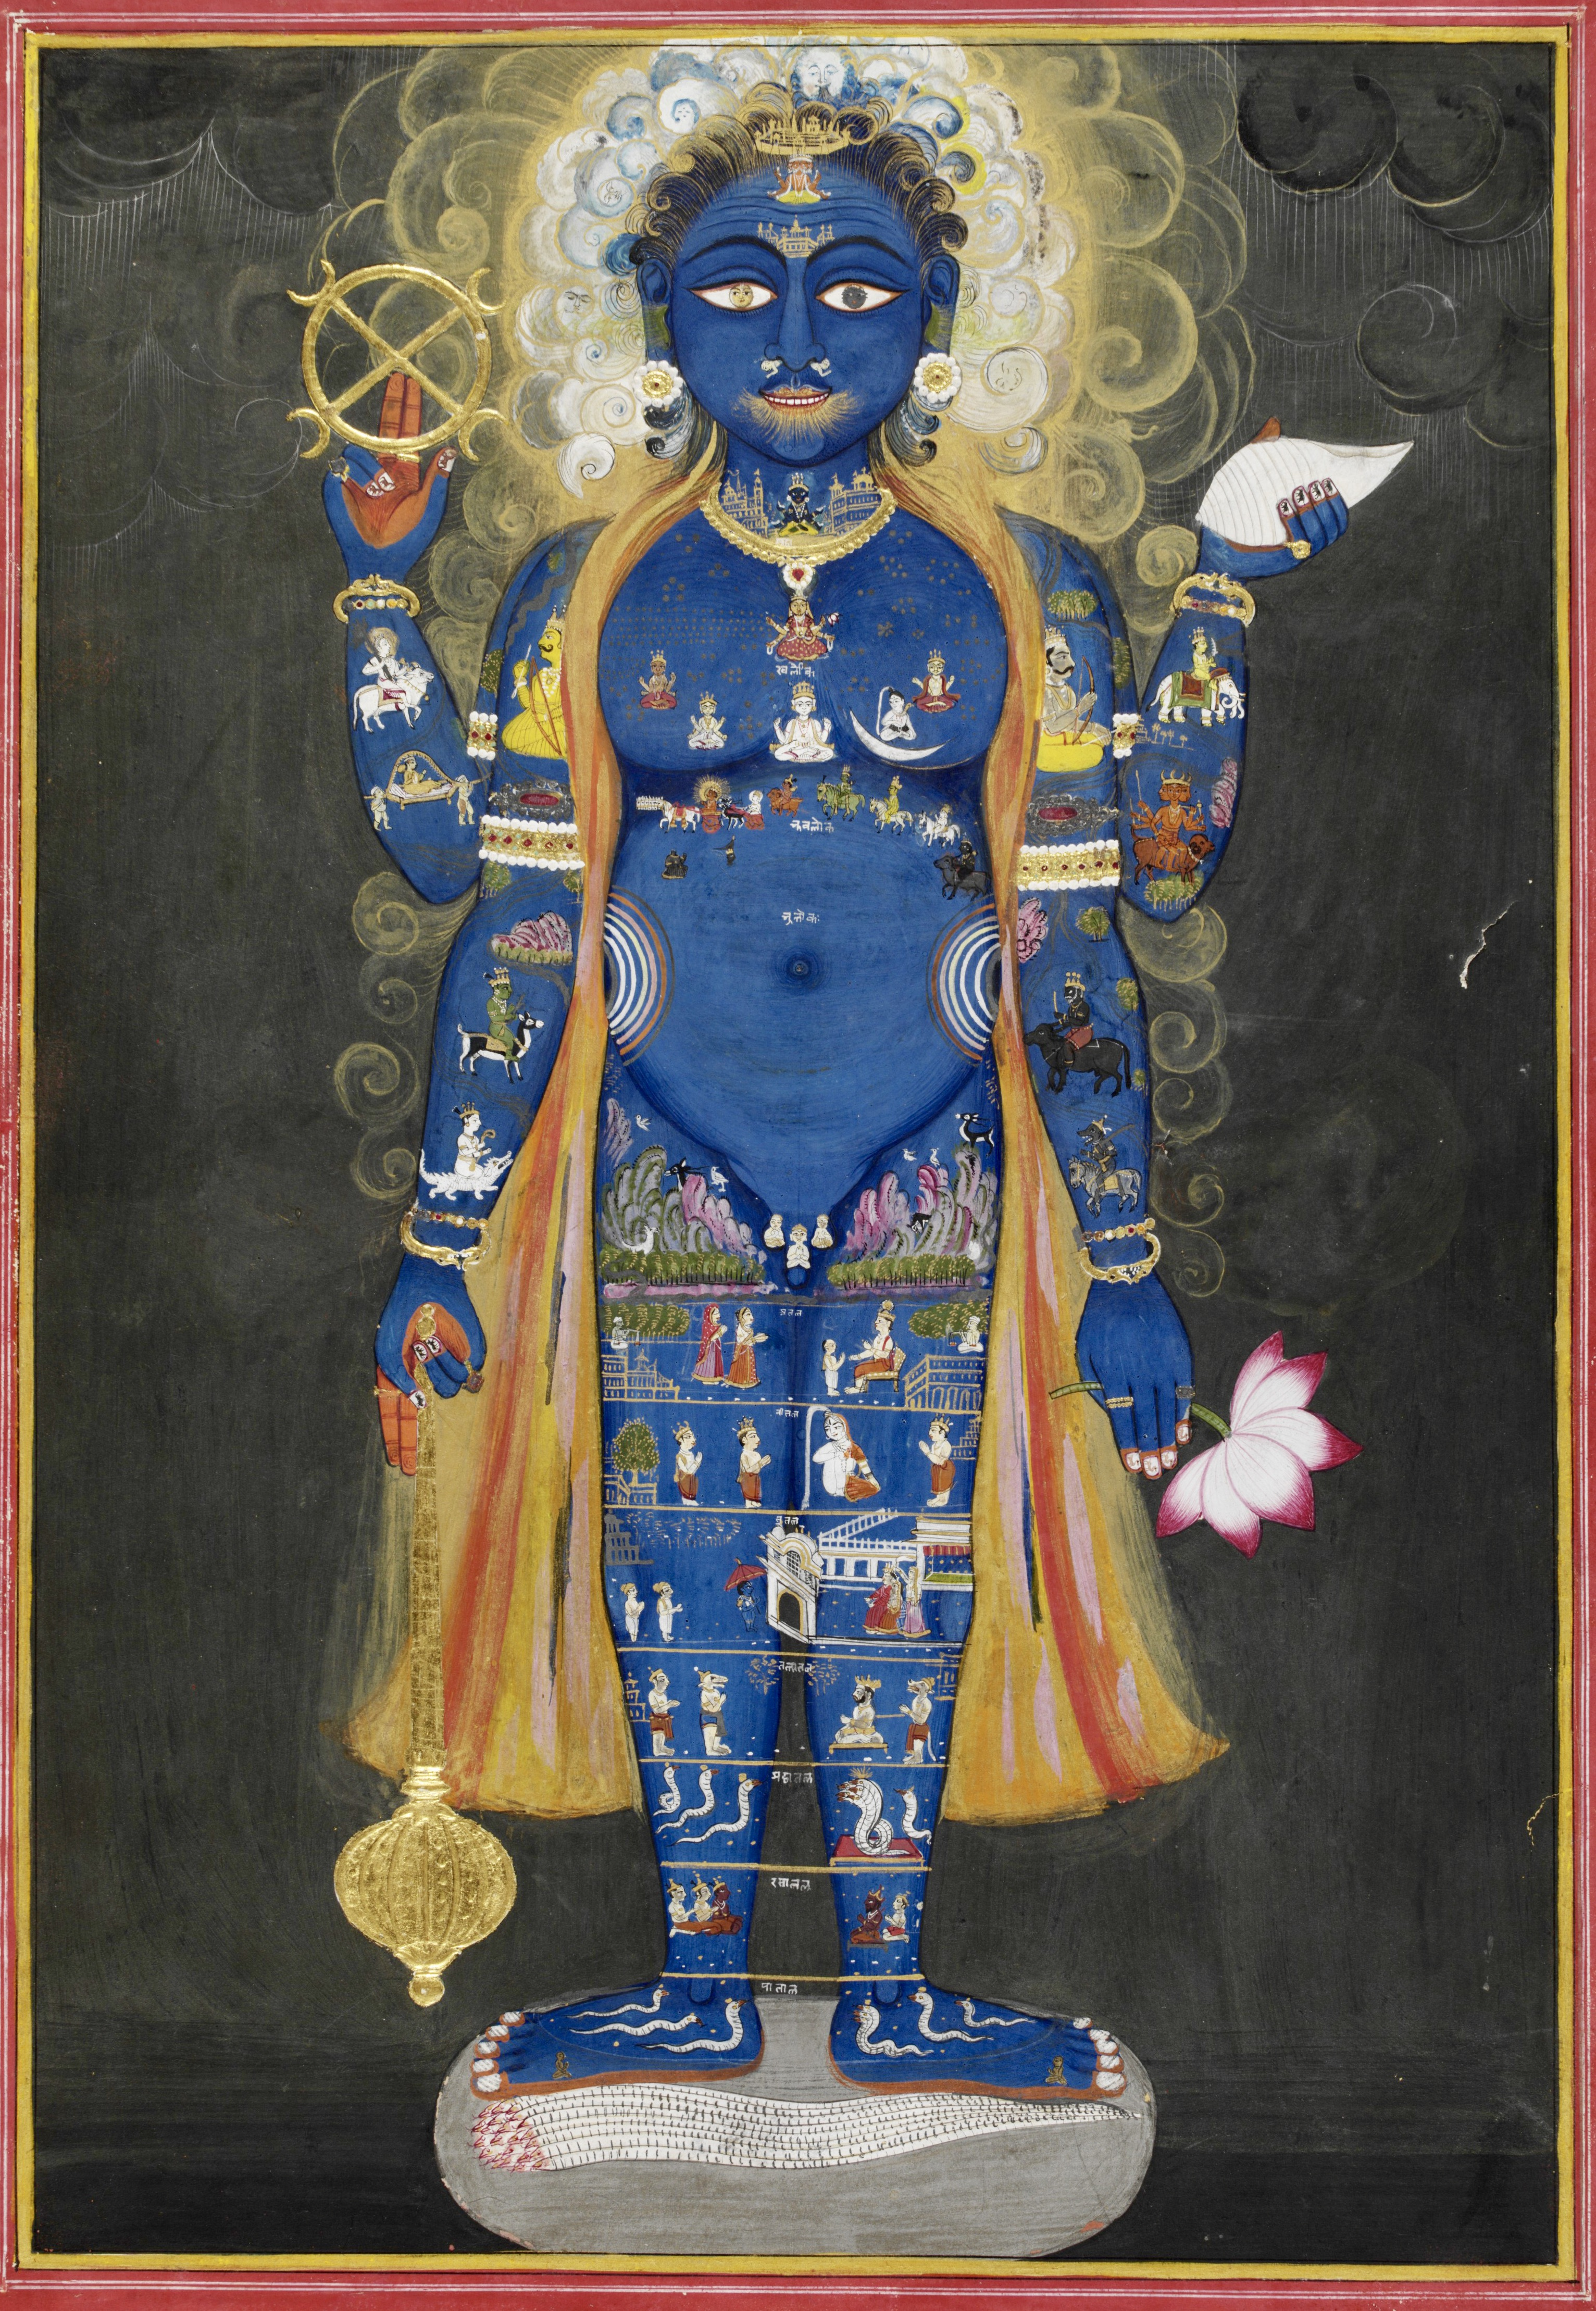
\includegraphics[width=1\textwidth]{pics/Vishnu_Vishvarupa_cropped.jpg}
	\caption{Viṣṇu Viśvarūpa, India, Rajasthan, Jaipur, ca. 1800–1820, Opaque watercolor and gold on paper, 38.5 × 28 cm, Victoria and Albert Museum, London, Given by Mrs. Gerald Clark.}
	\label{fig1}
      \end{figure}
\clearpage
  \begin{figure}[ht]
	\centering
  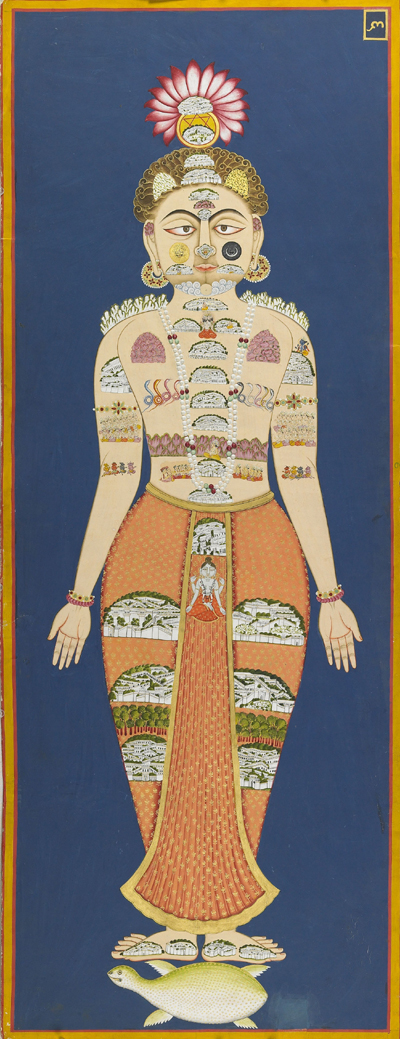
\includegraphics[width=0.5\textwidth]{pics/The_Equivalence_of_Self_and_Universe_(detail),_folio_6_from_the_Siddha_Siddhanta_Paddhati,_(Bulaki),_1824_(Samvat_1881);_122_x_46_cm._Mehrangarh_Museum_Trust..jpg}
	\caption{The Equivalence of Self and Universe (detail), folio 6 from the \textit{Siddhasiddhāntapaddhati} (Bulaki), India, Rajasthan, Jodhpur, 1824 (Samvat 1881), 122 x 46 cm, RJS 2378, Mehragarh Museum Trust.}
	\label{fig2}
      \end{figure}
      % \end{landscape}


\chapter{Bibliography}
 \label{sec:bibli}
   \clearpage
\newpage 
\thispagestyle{empty}
\quad  \addtocounter{page}{-1}

\printbibliography[heading=subbibintoc, title=Consulted Manuscripts, keyword=codex]

\printbibliography[heading=subbibintoc, title=Printed Editions, keyword=printsource]

\printbibliography[heading=subbibintoc, title=Secondary Literature, keyword=seclit]

\printbibliography[heading=subbibintoc, title=Online Sources, keyword=onlinesource]

\end{document}
